\documentclass[12pt,a4paper]{article}
\usepackage{graphicx}
\usepackage{caption}
\usepackage{natbib}
\usepackage{afterpage}
\def\conj#1{{#1^*}}
\def\im#1{{\mathrm{Im}(#1)}}
\def\re#1{{\mathrm{Re}(#1)}}
\def\lapl#1{{\mathrm{\bf L\!T}({#1})}}
\def\ztrans#1{{\mathrm{\bf Z\!T}(#1)}}
\def\sampl#1{{\widehat{#1}}}
\def\dt{{\mathrm{dt}}}
\def\R{\mathrm{R\!\!\!\!\!I}}
\def\C{\mathrm{{\bf C\!\!\!\!I}}}
\usepackage{hyperref}
\hypersetup{%
    pdfborder = {0 0 0}
}
\hypersetup{
    colorlinks,
    citecolor=blue,
    filecolor=blue,
    linkcolor=blue,
    urlcolor=blue
}
\renewcommand{\familydefault}{\sfdefault}
\renewcommand{\captionfont}{\small}
%
%
%
%
%
%
%
%
%
%
\begin{document}

\begin{center}
\mbox{\includegraphics[width=\textwidth]{SchEng_mono}}

\vfill

{\bf \Huge Digital Signal Processing}

\bigskip

{\Large Bernd Porr \& Nick Bailey}

\bigskip

{\small \today}

\vfill

\url{https://www.youtube.com/dspcourse}

\bigskip

\noindent\texttt{Attribution-ShareAlike 4.0 International (CC BY-SA 4.0)}

\vfill


\end{center}

\clearpage

\tableofcontents

\clearpage

\section{Acknowledgements}
A big thanks to Fiona Baxter for typing up the handwritten lecture notes and turning
them into \LaTeX.

\section{Introduction}
This handout introduces you into the basic concepts of Digital Signal Processing.
In contrast to the YouTube clips it focusses more on the theoretical
aspects of it and its analytical derivations. The (video-) lectures
cover more practical programming examples in Python and C++.

\subsection{Suggested reading}
\begin{itemize}
\item Digital Signal Processing
by John G. Proakis and Dimitris K Manolakis
\item Digital Signal Processing: System Analysis and Design by Paulo S. R. Diniz, Eduardo A. B. da Silva, and Sergio L. Netto 
\end{itemize}

\subsection{Advantages of digital signal processing}
\begin{itemize}
\item flexible: reconfigurable in software!
\item easy storage: numbers!
\item cheaper than analogue design
\item very reproducible results (virtually no drift)
\end{itemize}

\subsection{Development boards}
Buy a DSP development board and play with it. You get them either
directly from a company or from a distributor such as Farnell or RS.
Also general purpose boards such as the Raspberry PI and Arduino are great
platforms for DSP.

\section{Python}
Python is a fully featured scripting language and it's very well
thought through in its approach. It has a vast library of modules
which means that only rarely you need implement low level
functionality. It can be programmed both in a quick and dirty approach
to try out new ideas and at the same time it supports object oriented
programming so that truly professional programs can be
developed.

Python has a straightforward interface to call C and C++ functions so
that you can also mix it with C/C++ to speed up processing. For
example a digital filter class might have the design parts written in python
and the actual fast filter routines implemented in C. All this is
supported by the python package management so that you can also deploy
mixed python / C code without any problems. For example the AI library by
google ``tensorflow'' can be installed as a python package and in the
background it uses the GPUs on your computer without even noticing.

Here, I just comment on certain aspects of Python which are
important for DSP. Check out the full documentation of python
if you are interested beyond DSP in it. In particular it has
also very easy to use support for GUI programming.

\subsection{How to use Python?}
There are two ways to use Python. The one is interactive within
the python console and then the other method is by running
a python script.

Development environments such as anaconda have both the
console and then scripting facility integrated under one
roof.

\paragraph{The python console}
The python console you can just start by typing
``python'':
\begin{verbatim}
Python 3.8.10 (default, Jun  2 2021, 10:49:15) 
[GCC 9.4.0] on linux
Type "help", "copyright", "credits" or "license" for more information.
>>> 
\end{verbatim}
then you can type in commands one by one. Under Windows you might
need to point the PATH variable to your python program or you let Anaconda
do it for you.

\paragraph{Python scripts}
Scripts are text files which contain python commands. One command
per line and these are executed line by line.

Write your commands in any text editor and save it as a
.py-file. However, it's recommended to use an editor which supports at
least python's indentation which is a very important feature of python.
We'll see that indentation in python
defines the body of a function, the content of a loop or the code
executed conditionally.

So, it's recommended for any serious
work to install an editor which supports python such as spyder, VS-code, py-charm
or emacs.

Once you have your script file saved just type ``python myscript.py''
and it will be executed.

\paragraph{Help}
There is an abundance of online help available for Python. The
official Python pages have an excellent tutorial
(\texttt{https://docs.python.org/3/tutorial/}) and of course you find
answers to all your questions on Stack Overflow.

If you need help for a function you can use the in built help function
``help(thecommand)'' to get help for ``thecommand''. Try out ``help(print)''
to get help for the ``print'' command.

\subsection{Packages/Modules}
The power of Python comes form thousands of modules which are shipped
with python or can be installed via python's package
manager. A package contains usually many modules.
The standard package manager of python is called ``pip''
which downloads the package for you and installs it. This is not just
very convenient but also is safe because the download location is the
official python repository.

In general you import modules with the ``import'' command. For example
``import numpy as np'' imports the module numpy into python and
abbreviates it as ``np'' so that you'd write ``np.sin(c)'' to call the
sine function in numpy.

The import command loads essentially a file
called ``numpy.py'' so that you can write your own modules just by
creating file with that name. See below in the ``class'' section for
an example. There are numerous ways how to import modules but the
``import as'' way is by far the most popular.

Important modules are:
\begin{itemize}
\item numpy: Numerical operations for number crunching, matrix/array
  operations, trigonometric functions, etc. It offers fast numerical
  operations on arrays and matrices. It also has extensive Fourier
  Transform commands.
\item pylab: Plotting functions (MATLAB style), statistics and data fitting functions
\item scipy: Scientific computing package. In particular we are insterested in
  scipy.signal which contains all the signal processing functions and
  filter design commands. It also offers Fourier Transforms, data io routines,
  vector quantisation, linear algebra, optimisation tools and statistics.
\end{itemize}


\subsection{Data types}
Python has all the standard data types such as int, float, string,
\ldots and a few more. You can check which type a variable has with:
``type(variable)''. Important for DSP are these types:

\paragraph{Numbers}
Numbers are represented in a standard way, including complex numbers:
\begin{itemize}
\item \texttt{6E23}$=6\cdot 10^{23}$
\item \texttt{6+2j} is a complex number which is just generated
  by adding a ``j'' to the imaginary part.
\item \texttt{complex(0,1)} creates 1j and is useful if you have
  variables which you want to combine into a complex number.
\end{itemize}
Note that python has implicit types which might make you trip
over. If you write ``a=1'' then ``a'' is an integer whereas
``a=1.0'' is a floating point number. You can force a certain type by using
the typecast operator, for example `` a = int(b)'' to create an integer.

\paragraph{Lists}
There are numerous data types in Python which allow storing
collections of data. For DSP we need: lists, tupels and arrays. To clear
up the confusion from the start we are going through them one
by one. First up: lists!
\begin{itemize}
\item \texttt{p~=~[1,9,77]} is a list with the components 1,2 and 77.
\item \texttt{p[2]} returns the third element of the list (the index
  counts from 0). Note the index needs to be an integer so you might
  need to cast a floating point variables first into an integer, for example
  ``p[int(a)]''.
\item \texttt{p[1:5]} extracts from the list all elements from
  index number 1 to index number 4 (!). The index 5 is excluded!
  This is called splicing. Check out the online docs
  for more examples.
\item \texttt{p~=~range(1,4)} generates $1, 2, 3$ which is the same as
  a ``for loop'' in C: for(int i=1;i<4;i++)
\item \texttt{p.append(10)} adds a new element to the end of the
  list. You see that lists are essentially classes with methods (see below)!
  Check out the documentation for more options to manipulate lists.
\item \texttt{len(p2)} provides the number of elements.
\end{itemize}

\paragraph{Tupels}
Tupels are similar to lists but they are rather used as
``containers'' to package up different variables into one variable. For
example, you might want to put the sampling rate and the resolution of
an ADC into a tuple as they belong together.
\begin{itemize}
\item \texttt{p~=~(1,9,'kk')} is a tupel with the two integer numbers 1,2 and 'kk'.
\item The round brackets are often omitted:
  \texttt{p~=~1,9,'kk'} which implicitly defines a tupel.
\item \texttt{p[1]} returns the 2nd element of the tupel (the index
  counts from 0).
\item Extracting a tupel into separate variables also works:
  \texttt{a,b,c = p} assigns 1 to a, 9 to b and 'kk' to c. This
  is very convenient for functions if you want to return more than
  one result. Just package them up into a tuple and return it.
\end{itemize}

\paragraph{numpy Arrays/Matrices}
Numpy arrays or matrices are used for number crunching and are ideal for
DSP. Use these for all of you DSP data manipulation.
They are essentially C arrays with a thin wrapper around
them. In order to create and manipulate these arrays you need to use the numpy functions.

\begin{itemize}
\item\texttt{a = np.array([1, 2, 5])} which creates a numpy
  array from a standard Python list containing 1,2,5.
\item\texttt{b = np.array([[6, 2], [9, 7]])} creates a two dimensional
  array.
\item There are a lot of convenience functions in numpy to create
  arrays just containing zeros, ones or ascending numbers etc. Check out
   the numpy docs.
\end{itemize}

Since numpy arrays are close relatives to C arrays they have an additional
field which is called ``dtype'' which determines the type of the
array elements, for example ``int16'' (a 16 bit wide integer).
\begin{verbatim}
>>> data
array([-12288, -12545, -12798, ...,    511,    513,    513], dtype=int16)
>>> data.dtype
dtype('int16')
>>> data.astype(float)
array([-12288., -12545., -12798., ...,    511.,    513.,    513.])
\end{verbatim}
where the member function ``astype'' can convert from one array type to another, here
from int16 to floating point.


\subsection{Control structures}

\paragraph{Conditionals}
Conditional operation is done in exactly the same way as in other languages:
\begin{verbatim}
if a > c:
    a = c
    c = c*2
print(c)
\end{verbatim}
The indent of 4 characters indicates the conditionally executed commands. The same
applies for do and while loops where the body has an indent. Here, print(c)
is always executed because it doesn't have an indent.

\paragraph{Loops}
Imagine you want to calculate the average of the array \texttt{y}.
\begin{verbatim}
s = 0.0
for i in range(len(y)):
    s = s + y[i]
print("Average:",s/len(y))
\end{verbatim}
The ``for'' statement iterates through all elements of an array with
the help of a list created by the ``range'' command. This is very much
C-like. However Python, as for example in C++11 or Swift, allows iterating over the array elements
themselves:
\begin{verbatim}
s = 0.0
for v in y:
    s = s + v
print("Average:",s/len(y))
\end{verbatim}
which is a much more compact and safe way of coding as there will
never be an out of bounds error.

Important: the \textsl{indent} indicates the commands which the loop
iterates through. This is the general rule in python.

See the Python documentation for other ways of creating loops.


\subsection{Functions}
Function definitions can happen anywhere in the program or in a separate file.
For example, the above average calculations can be defined as:

\begin{verbatim}
def myaverage(y):
    s = 0.0
    for v in y:
        s = s + v
    return (s/len(y))
\end{verbatim}
and then called from the main program as \texttt{myaverage(a)}.  The
keyword ``def'' indicates the start of the function definition.  Note
again the 4 character indent for the function body and the colon after
the function name. This is characteristic for python.


\subsection{Classes}
Classes contain functions and variables. They usually
have a constructor called \texttt{init} which is a special function which is called
when an instance of a class is created.
\begin{verbatim}
class MyAmazingClass:
    def __init__(self,coeff):
        # Your init code here.
        self.mylocalcoeff = coeff

    def doSomeProcessing(self,data):
        # we process data
        data = data * self.mylocalcoeff
        return data
\end{verbatim}
(!) Note the special variable ``self'' which is \textsl{the first}
argument of every method in a class. Variables which
are part of the class are references by ``self''. For
example the constructor argument ``coeff'' is saved
in the class as ``mylocalcoeff'' and is then available
throughout the lifetime of the class as ``self.mylocalcoeff''. When we call
the method ``doSomeProcessing'' then ``self.mylocalcoeff''
is multiplied with the ``data'' argument and the result
is returned. Anything which hasn't got ``self.'' in front
of it will be forgotten after the function has terminated.
In this way you distinguish which variables are kept
for the lifetime of the class or
are just used temporarily.

Classes are just types and need to be instantiated:
\begin{verbatim}
f = MyAmazingClass(5)
a = f.doSomeProcessing(10)
b = f.doSomeProcessing(20)
\end{verbatim}
which will give us 50 as a result for the variable ``a'' and
100 for the variable ``b''. The variable ``f'' is the instance
of the class MyAmazingClass and the argument initialises
self.mylocalcoeff with 5.


\subsection{Mathematical functions}
Just import the numpy library which contains all the
mathematical functions and constants such as pi.
\texttt{import numpy as np}. It has all the standard functions such
as np.sin, np.cos, np.tan, np.exp, \ldots.

Note that these functions also take arrays as arguments. For example,
inputting the array x into the sine:
\begin{verbatim}
x = np.array(range(6))
y = np.sin(x);
\end{verbatim}
yields again an array in y! All elements have been processed at the 
\emph{same} time.


\subsection{Plotting of Functions}
Pylab has a vast amount of plotting functions which supports simple plotting
with just two commands (plot and show) up to complex animations of 3D data.
Plotting a sine wave can be achieved with:
\begin{verbatim} 
import matplotlib.pyplot as plt
import numpy as np
x = np.linspace(0,2*np.pi,100)
y = np.sin(x)
plt.plot(x,y)
plt.show()
\end{verbatim}
where I have used the numpy linspace command to create an array which
runs from 0 to two pi with 100 samples.

If you want to create more plot-windows you can use the command
\texttt{plt.figure}. Access the windows with the commands \texttt{plt.figure(1)},
\texttt{plt.figure(2)}.

It is also possible to combine plot windows into one with the
command \texttt{subplot}.

How to make it look nice? Here is an example:
\begin{verbatim}
plt.xlabel('time (s)')
plt.ylabel('voltage (V)')
plt.title('That is an AC voltage over time!')
plt.grid(True)
\end{verbatim}

Generally the best approach is to use an example and then customise it to your needs.




\subsection{Importing data}

\paragraph{Space/Tab/Comma separated data}
Numpy has a very handy import function for data as long as the the
elements in the data file are separated with spaces, tabs or
commas. To load such data files just type in: \texttt{x =
  np.loadtxt('mydatafile.dat')}. This creates a two dimensional array
which reflects exactly the structure in the datafile.

Thus, if you want to write software which creates Python
readable data then just export the data as space/tab separated ASCII files.



\paragraph{WAV files}
Scipy contains in its submodule io a subsubmodule wavfile which supports
reading and writing wav files:
\begin{verbatim}
import scipy.io.wavfile as wavfile
fs,data = wavfile.read('kongas.wav');
\end{verbatim}
fs,data is a tuple containing the sampling rate and then the data.

\begin{verbatim}
import scipy.io.wavfile as wavfile
wavfile.write('kongas_filt.wav',fs,y3);
\end{verbatim}
whereas 'fs' is the sampling rate and y3 the data -- usually normalised between
-1 and +1 for floating point numbers.


\clearpage


\section{Signal conversion}

We start with a few definitions when we transform an analogue signal into the digital
domain and back:

\begin{enumerate}

\item {\bf Sampling}

\begin{equation}
\underbrace{x_{a}(nT)}_{\mbox{analogue signal}}~ \equiv \underbrace{x(n)}_{\mbox{discrete data}}
\end{equation}

\begin{itemize}
\item $x_a(t)$: analogue signal
\item $T$: sampling interval, $\frac{1}{T}=F_s$ is the sampling rate
\item $x(n)$: discrete data
\end{itemize}

\item {\bf Quantisation} 
Continuous value into discrete steps. $x(n) \rightarrow x_{q}(n)$

\item {\bf Coding}
$x_{q}(n) \rightarrow$  into binary sequence or integer numbers.
\end{enumerate}


\subsection{Sampling}
The analogue signal $X_a$ is sampled at intervals $T$ to get
the sampled signal $X(n)$.
\begin{equation}
x(n) = x_{a}(nT),  \qquad -\infty < n < +\infty
\end{equation}

\subsubsection{Normalised frequency}
Note that the sampling frequency
\begin{equation}
F_{s} = \frac{1}{T_s}
\end{equation}
is lost and needs to be stored additionally so that the analogue
signal can be reconstructed:
\begin{equation}
x_{a}(t) = x_{a}(nT) = x_{a}(\frac{n}{F_{s}})
\end{equation}

\begin{figure}[!hbt]
\begin{center}
\mbox{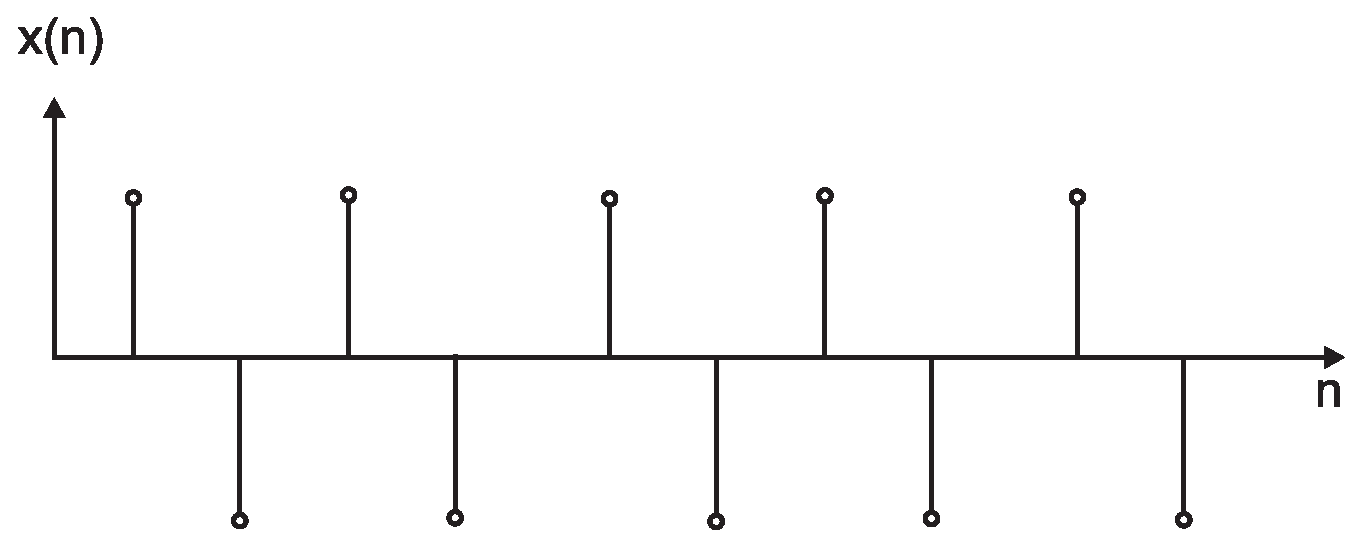
\includegraphics[width=0.75\textwidth]{max_sampl}}
\end{center}
\caption{Maximum frequency of a sampled signal is half the
normalised frequency.
\label{max_sampl}}
\end{figure}


What is the frequency range of our digital signal? What is
the maximum frequency in digital terms? Fig~\ref{max_sampl} shows that the
max frequency is $0.5$ because we need two samples to
represent a ``wave''. The frequency range $0\ldots 0.5$
is called the \textsl{normalised frequency} range. What is the relation
between normalised frequency and sampling rate?

Let's have a look at the analog signal $X_{a}(t)$ with the frequency $F$:
\begin{equation}
x_{a}(t) = A\cos (2\pi F t)
\end{equation}
and we sample it only at:
\begin{equation}
t = n/F_s
\end{equation}
Then the digital signal is:
\begin{equation}
x_{a}(n) = A \cos (2 \pi F/F_s n)
\end{equation}

Now, we can define the normalised frequency as:
\begin{equation}
\mbox{Normalised frequency:} \qquad f =  \frac {F}{F_s}
\end{equation}
which has its max value at $0.5$ which represents one period of
a sine wave within two samples\footnote{Note that the normalised
frequency in Python's scipy is differently defined. In scipy it is
annoyingly defined as $f_{\mbox{scipy}} =  2 \frac {F}{F_s}$. So, in other
words $f_{\mbox{scipy}}=1$ is the Nyquist frequency instead
of $f=0.5$ as normally defined.}


\subsubsection{Nyquist frequency}
Recall that the max value for the normalised frequency $f$ is $0.5$
and that:
\begin{equation}
x_{a}(n) = A \cos (2 \pi n f)
\end{equation}
with $n$ as an integer because
we are sampling.

What happens above $f>0.5$? Imagine $f = 1$
\begin{equation}
x_{a}(n) = \cos (2 \pi n) = 1 \qquad f=1
\end{equation}
which gives us DC or zero frequency. The same is true for
$f = 2, 3, 4, \ldots$. We see that above $f=0.5$ we never
get higher frequencies. Instead they will always stay between
$0\ldots 0.5$ for the simple reason that it is not possible
to represent higher frequencies. This will be discussed later
in greater detail.

The ratio $F/F_s$ must  be lower than $0.5$ to avoid ambiguity
or in other words the maximum frequency in a signal must be lower than 
$\frac{1}{2} F_s$. This is the Nyquist frequency.

If there are higher frequencies in the signal then these frequencies
are ``folded down'' into the frequency range of $0\ldots \frac{1}{2} F_s$
and creating an alias of its original frequency in the so called
``baseband'' ($f=0\ldots 0.5$). As long as the alias is not overlapping
with other signal components in the baseband this can be used to
downmix a signal. This leads to the general definition of the
sampling theorem which states that the bandwidth $B$ of the input signal
must be half of the sampling rate $F_s$:
\begin{equation}
B < \frac{1}{2}F_s
\label{samplingTheorem}
\end{equation}
The frequency $\frac{1}{2}F_s$ is called the Nyquist frequency.

\begin{figure}[!hbt]
\begin{center}
\mbox{\includegraphics[width=0.75\textwidth]{anti_alias}}
\end{center}
\caption{Anti alias filtering. A) with a lowpass filter. B)
with a sigma delta converter with very high sampling rate.
\label{anti_alias}}
\end{figure}

What do we do if the signal contains frequencies above 
$\frac{1}{2} F_s$? There are two ways to tackle this problem:
The classical way is
to use a lowpass filter (see Fig.~\ref{anti_alias}A) which filters
out all frequencies above the Nyquist frequency. However this
might be difficult in applications with high resolution A/D converters.
Alternatively one can use a much higher sampling rate to avoid
aliasing. This is the idea of the sigma delta converter
which operates at sampling rates hundred times higher than the
Nyquist frequency.


\subsubsection{Sampling theorem}
Is it possible to reconstruct an analogue signal from a digital signal
which contains only frequencies below the Nyquist frequency?

\begin{equation}
F_s > 2 F_{\mbox{max}}
\end{equation}
where $F_{\mbox{max}}$ is max frequency in the signal which we
represent by sine waves:
\begin{equation}
x_{a}(t) = \sum_{i=1}^{n} A_i \cos (2 \pi F_{i}t  + \Theta_{i})
\end{equation}

The analogue signal $x_{a}(t)$ can be completely reconstructed if:
\begin{equation}
g(t) = \frac{\sin 2\pi Bt}{2 \pi Bt}
\end{equation}

with
\begin{equation}
B = F_{\mbox{max}}
\end{equation}

\begin{equation}
x_{a}(t) = \sum_{h= -a}^{a}x_{a}(\frac{n}{F_s})g(t - \frac{h}{F_s})
\end{equation}

The problem is that $g(t)$ runs from negative time to positive time
and as we see later is a-causal so that this cannot be implemented
for real but approximations of $g(t)$ are possible and are analogue
lowpass filters which smooth out the step like outout of an digital
to analogue converter.



\subsection{Quantisation}
\begin{figure}[!hbt]
\begin{center}
\mbox{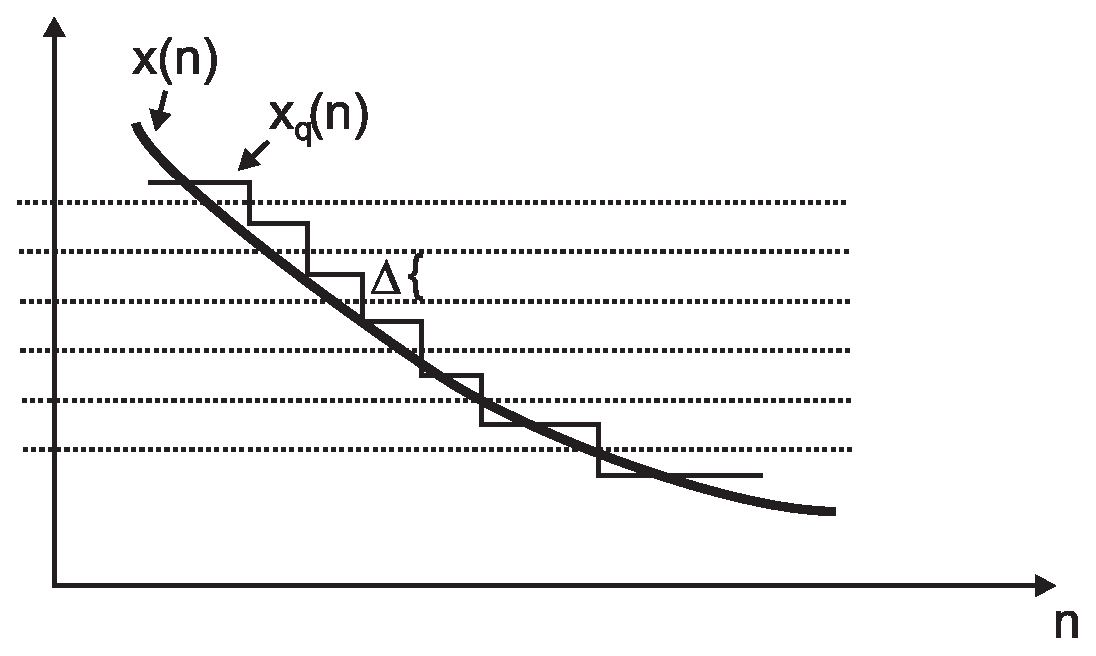
\includegraphics[width=0.75\textwidth]{quant_overv}}
\end{center}
\caption{$\Delta$ is the quantisation step.
\label{quant_overv}}
\end{figure}
A/D converters have a certain resolution. For example, the MAX1271 has a
resolution of 12 bits which means that it divides the input range into
4096 equal steps (see Fig~\ref{quant_overv}).
\begin{equation}
\Delta = \mbox{quantisation step} = 
\frac{x_{\mbox{max}} - x_{\mbox{min}}}{L - 1}
\end{equation}
where $x_{\mbox{max}} - x_{\mbox{min}}$ is the dynamic range in volt
(for example $4.096V$) and $L$ is the number of quantisation steps
(for example, 4096). $\Delta$ is the quantisation step which defines
minimal voltage change which is needed to see a change in the output
of the quantiser. The operation of the quantiser can be written down
as:
\begin{equation}
x_{q}(n) = Q[x(n)]
\end{equation}

\begin{figure}[!hbt]
\begin{center}
\mbox{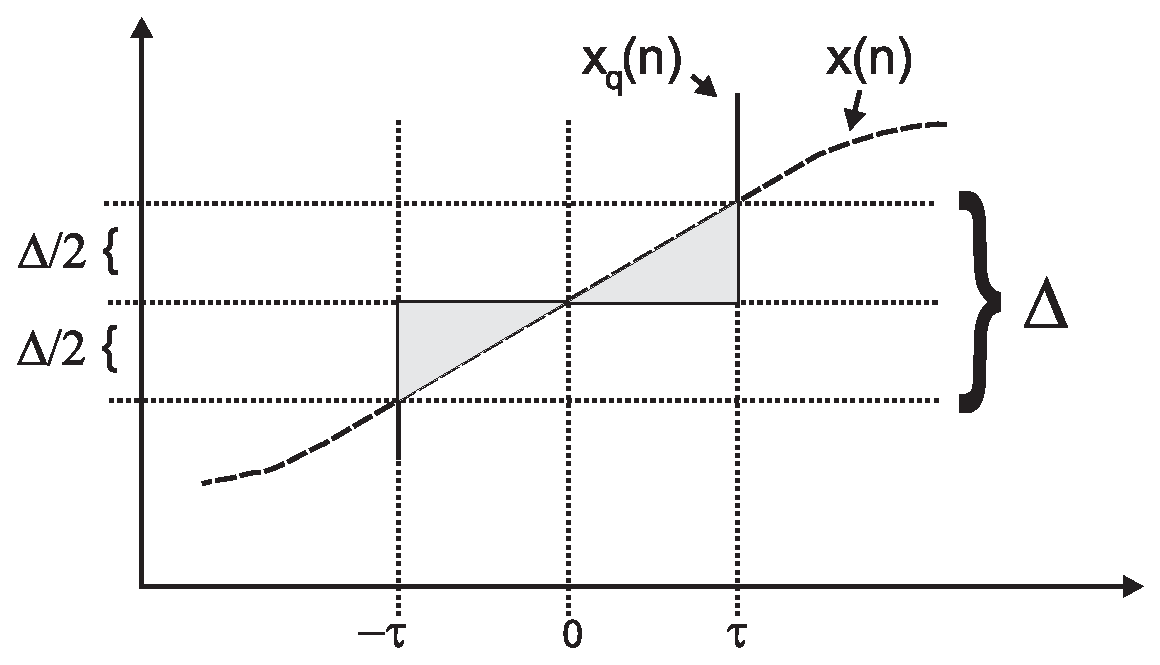
\includegraphics[width=0.75\textwidth]{quant_err}}
\end{center}
\caption{Illustration of the quantisation error. It is zero at $t=0$
and increases to the edges of the sampling interval. Illustrated
is the worst case scenario. This repeats in the next sampling interval
and so forth.
\label{quant_err}}
\end{figure}

Fig.~\ref{quant_err} shows error produced by the quantiser in the
worst case scenario. From that it can be seen that the maximum quantisation
error is half the quantisation step:
\begin{equation}
- \frac{\Delta}{2} \le e(n) \le \frac{\Delta}{2}
\end{equation}
The smaller the quantisation step $\Delta$ the lower the error!

What is the mean square error $P_{q}$?
\begin{equation}
P_{q} = \frac {1}{\tau} \int_{0}^{\tau} e_{q}^{2}(t)  dt
\end{equation}

\begin{eqnarray}
P_{q} & = & \frac{1}{\tau} \int_0^\tau \left(\frac{\Delta}{2\tau}\right)^2 t^2 dt \\
      & = & \frac{\Delta^2}{4 \tau^3} \int_0^\tau t^2 dt
\end{eqnarray}

\begin{eqnarray}
P_{q} = \frac{\Delta^2}{12\tau^3} \tau^3 =\frac{\Delta^2}{12}
\end{eqnarray}

this then results in the almost trival result that the size of the
quantisation step $\Delta$ scales linarly with the average error $\sqrt{P_{q}}$. So if we
have two times more quantisation steps then the error will half!

What is the relative error to a sine wave?
\begin{equation}
P_x = \frac{1}{T_p} \int_{0}^{T_p}(A \cos \Omega t)^2 dt = \frac{A^2}{2}
\end{equation}

Ratio to signal power to noise:

\begin{eqnarray}
\mbox {SQNR} &=& \frac {P_x}{P_q} = \frac{A^2}{2} . \frac{12}{\Delta^2} \\
             &=& \frac{6A^2}{\Delta^2}
\end{eqnarray}
This equation needs to be interpreted with care because increasing
the amplitude of the input signal might lead to saturation if the
input range of the A/D converter is exceeded.





\section{Frequency representation of signals}
Often we are more interested in the frequency representation
of signals than the evolution in time.

We will use small letters for time domain representation
and capital letters for the frequency representation, for example
$X(F)$ and $x(t)$.

\subsection{Continuous time and frequency}

\subsubsection{Periodic signals}
Periodic signals can be composed of sine waves :
\begin{equation} 
x(t) = \sum_{k = -\infty}^{\infty} c_{k} e^{j2\pi k F_1 t}
\end{equation}
where $F_1$ is the principle or fundamental frequency and $k \neq 1$ are the
harmonics with strength $c_k$. Usually $c_1$ is set to $1$. This is a
Fourier series with $c_{k}$ as coefficients. For example an
ECG has a fundamental frequency of about 1Hz (60 beats per minute).
However, the harmonics give the ECG its characteristic peak like shape.

How do we find the coefficients $c_k$?
\begin{equation} 
c_{k} = \frac{1}{T_p} \int_{T_p} x(t) e^{-j2 \pi k F_1 t} dt
\end{equation}

For simple cases there are analytical solutions for $c_k$, for example
for square waves, triangle wave, etc.

What are the properties of $c_{k}$?
\begin{equation}
c_{k} = c_{- k}^{*} \qquad \Leftrightarrow \qquad x(t)\mbox{ is real}
\end{equation}
or
\begin{eqnarray}
c_{k} &=& \mid c_k \mid e^{j \theta_k} \\
c_{-k} &=& \mid c_k \mid e^{-j \theta_k}
\end{eqnarray}

Proof: with the handy equation\ldots
\begin{equation}
\cos z = \frac{1}{2} \left(e^{zi} + e^{-zi}\right)
\end{equation}
we get
\begin{eqnarray} 
x(t) & = & c_0 + \sum_{k = 1}^{\infty} \mid c_k \mid e^{j \theta_k} e^{j 2\pi k F_1 t}
               + \sum_{k = 1}^{\infty} \mid c_{k}\mid e^{-j \theta_k} e^{-j 2\pi k F_1 t} \\
     & = & c_0 + 2 \sum_{k = 1}^{\infty} \mid c_k \mid \cos(2 \pi k F_1 t + \theta_{k})
\end{eqnarray}



How are the frequencies distributed? Let's have a look at the
frequency spectrum of a periodic signal: $P_{k} = \mid c_{k} \mid^{2}$

\begin{itemize}
\item There are discrete frequency peaks
\item Spacing of the peaks is $\frac{1}{T_1} = F_1$
\item Only the positive frequencies are needed: $c_{-k} = c_{k}^{*}$
\end{itemize}



\subsubsection{A-periodic signals}
In case nothing is known about $X(t)$ we need to integrate
over all frequencies instead of just the discrete frequencies.
\begin{equation} 
X(F) = \int_{-\infty}^{\infty} x(t) e^{-j 2 \pi F t} dt
\end{equation}
Consequently, the frequency spectrum $X(F)$ is continuous.
\begin{equation} 
x(t) = \frac{1}{2\pi} \int_{-\infty}^{\infty} X(F) e^{j 2 \pi F t} dF
\end{equation}






\subsection{Sampled time and/or frequency}

\subsubsection{Discrete time Fourier Transform (DTFT)}

The signal $x(n)$ is discrete whereas the resulting frequency
spectrum is considered as continuous (arbitrary signals).

\begin{itemize}
\item Analysis or direct transform:
\begin{equation}
X(\omega)=\sum_{n=-\infty}^{\infty} x(n) e^{-j\omega n}
\end{equation}

\item Synthesis or inverse transform:
\begin{eqnarray}
x(n) & = & \frac{1}{2\pi} \int_{-\pi}^{\pi} X(\omega) e^{j\omega n} d\omega \\
     & = & \frac{1}{2\pi} \int_{-0.5}^{0.5} X(f) e^{j 2\pi f n} df
\end{eqnarray}
note the range here. $f$ is the normalised frequency.

\end{itemize}


\subsubsection{The effect of time domain sampling on the spectrum (Sampling
theorem)}
\begin{figure}[!hbt]
\begin{center}
\mbox{\includegraphics[width=0.75\textwidth]{periodic_ny}}
\end{center}
\caption{Effect of sampling on the spectrum.
\label{periodic_ny}}
\end{figure}
What effect has time domain sampling on the frequency spectrum\footnote{This derivation is loosely based on \citet{Proakis1996}}? Imagine we
have an analog spectrum $X_a(F)$ from a continuous signal $x(t)$. We want
to know how the spectrum $X(F)$ of the discrete signal $x(n)$ looks like.
\begin{equation}
X(F) \Leftrightarrow X_a(F)
\end{equation}
The signal is represented by $x(n)$ so that
we can equate the Fourier transforms of the sampled spectrum $X(F)$ and
of the analogue spectrum $X_a(F)$. 
\begin{equation}
\int_{-0.5}^{0.5} \underbrace{X(f)}_{\mbox{sampled}} e^{j 2 \pi f n} df = 
\int_{-\infty}^{+\infty} \underbrace{X_a(F)}_{\mbox{cont}} e^{j 2\pi n F/F_s} dF
\label{sampl_idea}
\end{equation}
Obviously $X(f)$ must be different to accommodate the different integration
ranges. The trick is now to divide the integral on the right hand side 
of Eq.~\ref{sampl_idea} 
into chunks to make it compatible to the range on the left hand
hand side.

Remember that the normalised frequency is $f=F/F_s$ which allows us
to change the integration to analogue frequency on both sides:
\begin{equation}
\frac{1}{F_s} \int_{-F_s/2}^{F_s/2} X(\frac{F}{F_s}) e^{j 2 \pi n F/F_s} dF
=
\int_{-\infty}^{+\infty} X_a(F) e^{j 2\pi n F/F_s} dF
\label{sampl_ana_dig}
\end{equation}
and now we divide the right hand side into chunks of $F_s$ which corresponds
to the integration range on the left hand side.
\begin{eqnarray}
\int_{-\infty}^{+\infty} X_a(F) e^{j 2\pi n \frac{F}{F_s}} dF
& = &
\sum_{k=-\infty}^{\infty} \int_{-\frac{1}{2} F_s + k F_s}^{+\frac{1}{2} F_s + k F_s} X_a(F) e^{j2\pi n \frac{F}{F_s}} dF \\
& = &
\sum_{k=-\infty}^{\infty} \int_{-\frac{1}{2} F_s}^{+\frac{1}{2} F_s} X_a(F-k F_s) \underbrace{e^{j2\pi n\frac{F}{F_s}}}_{k F_s \mbox{ omit.}} dF \\
& = &
\int_{-\frac{1}{2} F_s}^{+\frac{1}{2} F_s} \underbrace{\sum_{k=-\infty}^{\infty} X_a(F-k F_s)}_{=X(F) \mbox{ of Eq.~\ref{sampl_ana_dig}}} e^{j2\pi n\frac{F}{F_s}} dF
\end{eqnarray}
This gives us now an equation for the sampled spectrum:
\begin{eqnarray}
X(F/F_s) & = & F_s \sum_{k=-\infty}^{\infty} X_a(F-kF_s) \\
X(f) & = & F_s \sum_{k=-\infty}^{\infty} X_a[(f-k)F_s]
\end{eqnarray}
This equation can now be interpreted. In order to get the sampled
spectrum $X(F)$ we need to make copies of the analog spectrum
$X_a(F)$ and place these copies at multiples of the sampling rate
$F_s$ (see Fig.~\ref{periodic_ny}). This illustrates also the
\textsl{sampling theorem}: if the bandwidth of the spectrum is wider
than $F_s/2$ then the copies of the analogue spectrum will overlap and
reconstruction would be impossible. This is called aliasing. Note that
it is not necessary bad that the spectrum of the analogue signal lies
within the range of the so called ``base band'' $-F/2 \ldots F/2$. It
can also lie in another frequency range further up, for example $-F/2
+ 34 \ldots F/2 +34$ as long as the
\textsl{bandwidth} does not exceed $F_s/2$. If it is placed further up
it will automatically show up in the baseband $-F/2 \ldots F/2$ which
is called ``fold down''. This can be used for our purposes if we
want to down mix a signal.

\begin{figure}[!hbt]
\begin{center}
\mbox{\includegraphics[width=\textwidth]{fold_down}}
\end{center}
\caption{Mapping of frequencies in the analogue domain ($F$)
and sampled domain ($f$). $F_s$ is the sampling rate.
\label{fold_down}}
\end{figure}

With the insight from these equations we can create
a plot of how analogue frequencies map onto sampled frequencies.
Fig~\ref{fold_down} shows how the analogue frequencies $F_\textrm{analogue}$
map on the normalised frequencies $f_\textrm{sampled}$.
As long as the analogue frequencies are below $F_s/2$ the mapping
is as usual as shown in Fig~\ref{fold_down}A. 
Between $F_s/2$ and $F_s$ we have an inverse mapping:
an increase in analogue frequency causes a decrease in frequencies.
Then, from $F_s$ we have again an increase in frequencies starting
from DC. So,
in general if we keep a bandlimited signal within one of these
slopes (for example from $F_s \ldots F_s + 1/2 F_s$ as 
shown in Fig~\ref{fold_down}B) then we can
reproduce the signal.

This leads us to the generalised Nyquist theorem: if a bandpass
filtered signal has a bandwidth of $B$ then the minimum sampling
frequency is $F_s = 2B$.

\subsubsection{Discrete Fourier Transform (DFT)}
So far we have only sampled in the time domain. However, on
a digital computer the Fourier spectrum will always be a discrete
spectrum.

The discrete Fourier Transform (DFT) is defined as:
\begin{equation}
X(k) = \sum_{n=0}^{N-1} x(n) e^{-j2\pi kn / N} \qquad k=0,1,2, \ldots, N-1
\label{DFT}
\end{equation}
where $N$ is the number of samples in both the time and frequency domain.

The inverse discrete Fourier Transform (IDFT) is defined as:
\begin{equation}
x(n) = \frac{1}{N} \sum_{k=0}^{N-1} X(k) e^{j 2\pi kn/N} \qquad n=0,1,2,\ldots, N-1
\end{equation}

\begin{figure}[!hbt]
\begin{center}
\mbox{\includegraphics[width=0.75\textwidth]{time_alias}}
\end{center}
\caption{Effect of sampling in the frequency domain. The
inverse in the time domain $x(n)$ contains repetitions of
the original signal.
\label{time_alias}}
\end{figure}


What is the effect in the timedomain of this discretisation\footnote{This derivation is loosely based on \citet{Proakis1996}}? We start with
the continuous Fourier transform
and discretise it into N samples in the frequency domain:
\begin{equation}
X\left(\frac{2\pi}{N}k\right) = \sum_{n = -\infty}^{\infty} x(n) e^{-j\frac{2\pi}{N}kn} \qquad k = 0, \ldots, N-1
\end{equation}

Let's subdivide the sum into chunks of length $N$:
\begin{eqnarray}
X\left(\frac{2\pi}{N}k\right) 
& = &
\sum_{l = -\infty}^{\infty} \sum_{n=lN}^{lN+N-1} x(n)e^{-j \frac{2\pi}{N}kn} \\
& = & \sum_{l=-\infty}^{\infty} \sum_{n=0}^{N-1} x(n-lN) e^{-j \frac{2\pi}{N} kn} \\
& = & \sum_{n=0}^{N-1} \underbrace{\sum_{l=-\infty}^{\infty} x(n - lN)}_{\mbox{Periodic repetition!}} e^{-j \frac{2\pi}{N}kn}
\end{eqnarray}

We note the following:
\begin{itemize}
\item Ambiguity in the time domain
\item The signal is repeated every N samples
\end{itemize}
Practically this repetition won't show up because
the number of samples is limited to $N$ in the inverse transform.
However, for operations which shift signals in the frequency domain
it is important to remember that we shift a periodic time series. If
we shift it out at the end of the array we will get it back at the
start of the array.

\begin{figure}[!hbt]
\begin{center}
\mbox{\includegraphics[width=0.75\textwidth]{dft_example}}
\end{center}
\caption{Example of a DFT. The sampled signal $x(n)$ is
converted to the spectrum $X(k)$. Both have $N$ samples.
Note the redundancy: the spectrum is mirrored around $N/2$.
The first value $X(0)$ is the DC value of the signal. However
this is the only sample which is not mirrored.
\label{dft_example}}
\end{figure}
Fig.~\ref{dft_example} shows an example of a DFT. It is important
to know that the spectrum is mirrored around $N/2$. DC is represented
by $X(0)$ and the Nyquist frequency $F_s/2$ is represented by
$X(N/2)$. The mirroring occurs because the input signal $x(n)$
is \textsl{real}. This is important if one wants to modify the
spectrum $X(F)$ by hand, for example to eliminate 50Hz noise. One
needs to zero two elements of $X(F)$ to zero. This is illustrated
in this python code:
\begin{verbatim}
import scipy as sp
yf=sp.fft(y)
# the sampling rate is 1kHz. We've got 2000 samples.
# midpoint at the ifft is 1000 which corresponds to 500Hz
# So, 100 corresponds to 50Hz
yf[99:101+1]=0;
# and the mirror
yf[1899:1901+1]=0;
#
yi=sp.ifft(yf);
\end{verbatim}
This filters out the 50Hz hum from the signal $y$ with sampling rate
1000Hz. The signal \texttt{yi} should be real valued again or contain
only very small complex numbers due to numerical errors.


\subsubsection{Properties of the DFT}
\begin{itemize}
\item Periodicity:
\begin{eqnarray}
x(n + N) & = & x(n) \\
X(k + N) & = & X(k)
\end{eqnarray}

\item Symmetry: if $x(n)$ real:
\begin{equation}
x(n)\mbox{ is real} \Leftrightarrow X^*(k) = X(-k) = X(N-k)
\end{equation}
This is important when manipulating $X(k)$ by hand.

\item Time Reversal:
\begin{eqnarray}
x(n) & \leftrightarrow & X(k) \\
x(-n)& \leftrightarrow & X(N - k)
\end{eqnarray}

\item \textsl{Circular} convolution:
\begin{equation}
X_{1}(k) X_{2}(k) \leftrightarrow x_1(n) * x_2(n)
\end{equation}
with
\begin{equation} 
x_{3}(m) = \sum_{n = 0}^{N - 1} x_{1}(n) x_{2}(m - n)
\end{equation}
\end{itemize}
More useful equations are at \citet[pp.415]{Proakis1996}.




\subsubsection{Problems with finite length DFTs}
\begin{figure}[!hbt]
\begin{center}
\mbox{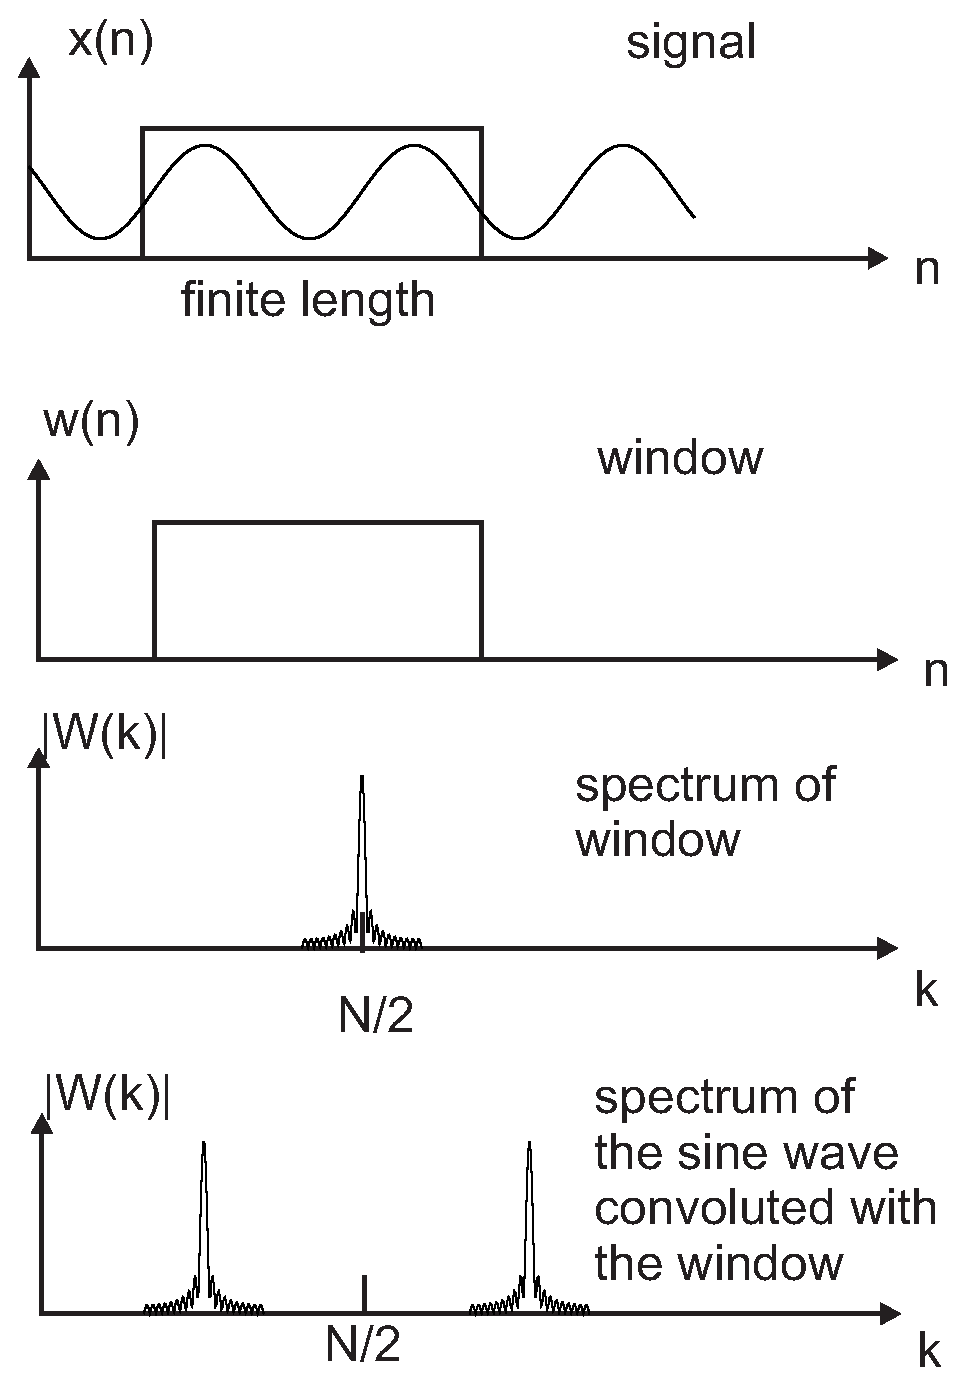
\includegraphics[width=0.75\textwidth]{windowing_dft}}
\end{center}
\caption{The effect of windowing on the DFT.
\label{windowing_dft}}
\end{figure}
\begin{equation}
x_w(n) = x(n) \cdot w(n)
\end{equation}
where $x$ is the input signal and $w(n)$ represents a function
which is $1$ from $n=0$ to $n=L-1$ so that we have $L$ samples
from the signal $x(n)$.

To illustrate the effect of this finite sequence we introduce a sine
wave $x(n) = \cos \omega_0 n$ which has just two peaks in a proper
Fourier spectrum at $-\omega$ and $+\omega$.

The spectrum of the rectangular window with the width $L$ is:
\begin{equation} 
W(\omega) = \frac{sin(\omega L /2)}{sin (\omega / 2)} e^{-j\omega (L -1)/2}
\end{equation}

The resulting spectrum is then:
\begin{equation} 
X_{3}(\omega) = X(\omega) * W(\omega)
\end{equation}

Because the spectrum of $X(\omega)$ consists of just two delta functions
the spectrum $X_{3}(\omega)$ contains the window spectrum $W(\omega)$ twice at
$-\omega$ and $+\omega$ (see Fig.~\ref{windowing_dft}). This
is called \textsl{leakage}. Solutions to solve the leakage problem?
Use Windows with a narrower spectrum and with less ripples
(see FIR filters).








\subsubsection{Fast Fourier Transform}

We can rewrite the DFT (Eq.~\ref{DFT}) in a slightly more compact form:
\begin{equation} 
X(k) = \sum_{n = 0}^{N-1}  x(n) W_{N}^{kn}
\label{compactDFT}
\end{equation}
with the constant:
\begin{equation} 
W_{N} = e^{-j 2\pi/N}
\label{constWN}
\end{equation}
The problem with the DFT is that it needs $N^2$ multiplications.
How can we reduce the number of multiplications?
Idea: Let's divide the DFT in an odd and an even sequence:
\begin{eqnarray}
& x(2m) & \\
& x(2m + 1), & \qquad m = 0, ..... , \frac{N}{2} - 1
\end{eqnarray}
which gives us with the trick $W_N^{2mk} = W_{N/2}^{mk}$ because of the
definition Eq.~\ref{constWN}.
\begin{eqnarray} 
X(k) & = & \sum_{m=0}^{N/2-1} x(2m) W_{N}^{2mk} + \sum_{m=0}^{N/2 - 1}  x(2m + 1) W_{N}^{k (2m + 1)} \\
& = & \sum_{m=0}^{N/2-1} x(2m) W_{N/2}^{mk} + W_{N}^{k} \sum_{m = 0}^{N/2 - 1} x(2m + 1) W_{N/2}^{mk} \\
& = & F_{e}(k) + W_{N}^{k} F_{o}(k)
\end{eqnarray}
$F_e$ and $F_o$ have both half the length of the original sequence and
need only $(N/2)^2$ multiplication, so in total $2 \cdot (N/2)^2 = \frac{N^2}{2}$.
Basically by dividing the sequence in even and odd parts we can reduce
the number of multiplications by 2. Obviously, the next step is then
to subdivide the two sequences $F_{e}(k)$ and $F_{o}(k)$ even further
into something like $F_{ee}(k), F_{eo}(k), F_{oe}(k)$ and $F_{oo}(k)$.

\begin{figure}[!hbt]
\begin{center}
\mbox{\includegraphics[width=0.75\textwidth]{fft_div}}
\end{center}
\caption{Illustration of the Fast Fourier Algorithm. The sequence
of $N$ samples is recursively divided into subsequences of odd and
even samples.
\label{fft_div}}
\end{figure}

In general the recipe for the calculation of the FFT is:
\begin{equation}
X_{i}(k) = X_{ie}(k) + W_{L}^{k} X_{io}(k)
\label{butterfly}
\end{equation}
$W_{L}^{k}$ is the phase factor in front of the odd sequence.
This is continued until we have only two point ($N=2$) 
DFTs (see Eq.~\ref{compactDFT}):
\begin{eqnarray}
\mbox{DC:} \qquad X(0) & = & x(0) + \underbrace{W_2^0}_{1} x(1) = x(0) + x(1) \label{dcDFT}\\
\mbox{Nyquist frequ.:} \qquad X(1) & = & x(0) + \underbrace{W_2^1}_{-1} x(1) = x(0) - x(1) \label{nyDFT}
\end{eqnarray}
A two point DFT operates only on two samples which can represent only
two frequencies: DC and the Nyquist frequency which makes the
calculation trivial. Eq.~\ref{dcDFT} is an averager and
Eq.~\ref{nyDFT} is basically a differentiator which gives the max output
for the sequence $1,-1,1,-1,\ldots$.  Fig.~\ref{fft_div} illustrates
how to divide the initial sequence to arrive at 2 point DFTs. In other
words the calculation of the full DFT is done by first calculating
$N/2$ 2 point DFTs and recombining the results with the help of
Eq.~\ref{butterfly}. This is sometimes called the ``Butterfly''
algorithm because the data flow diagram can be drawn as a butterfly.
The number of complex multiplications reduces in this approach to $N
\log_2 N$ which is actually the worst case scenario because many
$W_{L}^{k}$ usually turn out to be $1,-1,j,-j$ which are just sign
inversions or swaps of real and imaginary parts. A clever
implementation of this algorithm will be even faster.

In summary the idea behind the FFT algorithms is to divide the sequence
into subsequences. Here we have presented the most popular radix 2 algorithm.
The radix 4 is even more efficient and there are also algorithms
for divisions into prime numbers and other rather exotic divisions.
However, the main idea is always the same: subsample the data in a clever
way so that the final DFT becomes trivial.

\subsection{Software}
In \citet{NumericalRec2007} you'll find highly optimised C code
for Fourier transforms. Most Linux distros (Ubuntu, Suse, RedHat, \ldots)
come with an excellent FFT library called \texttt{libfftw3}.


\subsection{Visualisation}
\begin{figure}[!hbt]
\begin{center}
\mbox{\includegraphics[width=\textwidth]{visualisation}}
\end{center}
\caption{
An ECG signal in the time- and frequency domain.
\label{visualisation}}
\end{figure}
The Fourier spectrum is a complex function of frequency which cannot
be displayed in a convenient way. Usually the amplitude or magnitude
of the spectrum is of interest (see Fig.~\ref{visualisation}) which is calculated as the
absolute value $|X(F)|$ of the Fourier spectrum X(F). In addition
the phase might be of interest which is calculated as $\arg(X(F))$.
\begin{itemize}
\item Magnitude or Amplitude: $|X(F)|$
\item Phase: $\arg(X(F))$
\end{itemize}

\clearpage





\section{Causal Signal Processing}

In realtime systems and any system where data is processed as it
arrives the values of the future samples are not known. This is as in
an analogue system where we send for example a signal into an
amplifier and it needs to process it as it arrives. The amplifier
won't know if the next music track is Mozart or Jimmy Hendrix. It just
needs to react to what it's fed into it.

However, the Fourier Transform is \textsl{not real time}.  We need the
whole signal from the first to the last sample.  For that reason we
need to develop a new mathematical framework which we call ``Causal
Signal Processing''. These systems should ideally react to an incoming
signal as an analogue system does, namely as fast as possible with
little latency as possible.

In the next section we are now developing a mathematical
framework for causal digital signal processing. We draw
here heavily from analoge circuit design as this is by
its own nature performs realtime causal processing.


\subsection{Causality}
\begin{figure}[!hbt]
\begin{center}
\mbox{\includegraphics[width=0.75\textwidth]{causality}}
\end{center}
\caption{A causal system only \textsl{reacts} to it's input.
Causal signals only evolve in positive time. Per definition the
signal is zero for $t<0$.
\label{causality}}
\end{figure}
Fig.~\ref{causality} illustrates the concept of causality.
Causal systems cannot look into the future. They can only react
to a certain input. Causal signals are kept zero for $t<0$
per definition.

\begin{figure}[!hbt]
\begin{center}
\mbox{\includegraphics[width=0.75\textwidth]{convol}}
\end{center}
\caption{Illustration of the convolution. The shaded area
shows the integration for $t=1$.
\label{convolution}}
\end{figure}

\subsection{Convolution of Causal Signals}
After having defined causality we can define the convolution in continous time:
\begin{eqnarray} 
  y(t) & = & h(t) * x(t) = \int_{-\infty}^{\infty} h(t - \tau) x(\tau) d\tau \\
  y(n) & = & h(n) * x(n) = \sum_{n = -\infty}^\infty h(n) x(m - n)
\label{eqconv}
\end{eqnarray}
Note the reversal of integration of the function $h$. This
is characteristic of the convolution. At time $t=0$
only the values at $h(0)$ and $x(0)$ are evaluated 
(see Fig.~\ref{convolution}). Note
that both functions are zero for $t<0$ (causality!).
At $t>0$ the surface which is integrated grows as shown
in Fig.~\ref{convolution} for $t=1$.

What happens if $x(t)=\delta(t)$? Then Eq.~\ref{eqconv}:
\begin{equation} 
y(t) = \int_{-\infty}^{\infty} h(t - \tau) \delta(\tau) d\tau = h(t)
\label{convdelta}
\end{equation}
provides us with the function $h(t)$ itself. This will
be used later to determine the impulse response of the
filter.

\subsection{Laplace transform}
The Fourier transform is not suitable for causal systems
because it requires the whole signal from $-\infty < t < +\infty$.
What we need is a transform which works with continuous causal signals.
This is the Laplace transform:
\begin{equation} 
\lapl{h(t)} = H(s) = \int_{0}^{\infty} h(t) e^{-st} dt
\label{lapltrans}
\end{equation}
The Laplace transform has a couple of very useful properties:
\begin{itemize}
\item Integration: 
\begin{equation}
\int f(\tau) d\tau \Leftrightarrow \frac{1}{s} F(s)
\end{equation}
\item Differentiation:
\begin{equation}
\frac{d}{dt} f(t) \Leftrightarrow s F(s) 
\end{equation}
\item Shift:
\begin{equation}
f(t - T) \Leftrightarrow e^{-Ts} F(s)
\label{shiftOperation}
\end{equation}
Proof:
\begin{eqnarray}
\lapl{h(t - T)} & = &\int_{0}^{\infty} h\underbrace{(t - T)}_{causal} e^{-st} dt \\
& = & \int_{0}^{\infty} h(t) e^{-s(t + T)} dt \\
& = & \int_{0}^{\infty} h(t) e^{-st} e^{-sT} dt \\
& = & e^{-sT} \underbrace{\int_{0}^{\infty} h(t) e^{-st} dt}_{H(s)} \\
& = & e^{-sT} H(s)
\end{eqnarray}

\item Convolution:
\begin{equation} 
f(t) * g(t) \Leftrightarrow F(s) G(s)
\end{equation}
\end{itemize}




\subsection{Filters}
\begin{figure}[!hbt]
\begin{center}
\mbox{\includegraphics[width=0.75\textwidth]{filter}}
\end{center}
\caption{General idea of a filter and how to describe it:
either with its impulse response or with it's Laplace transforms.
\label{filter}}
\end{figure}
Fig.~\ref{filter} presents a causal filter as a black box in continuous time. We
send in a signal and and we get a signal out of it. The
operation of the filter is that of a convolution of the input
signal or a multiplication in the Laplace space:
\begin{equation} 
g(t) = h(t) * x(t) \Leftrightarrow Y(s) = H(s) \cdot X(s)
\end{equation}

\subsubsection{How to characterise filters?}

\begin{enumerate}
\item{\bf Impulse Response}
\begin{eqnarray}
x(t) & = & \delta(t) \qquad \leftarrow \mbox{delta pulse} \\
h(t) & = & y(t) \qquad \leftarrow \mbox{impulse response}
\end{eqnarray}
The filter is fully characterised by its impulse response $h(t)$

\item{\bf Transfer function}
The Laplace transform of the impulse response is called
\textsl{Transfer Function}. With the argument $j\omega$ we
get the frequency
response of the filter. What does the frequency response tell us about
the filter?  The absolute value of the
\begin{equation}
|H(i \omega)|
\end{equation}
gives us the amplitude or magnitude for every frequency
(compare the Fourier transform).
The angle of the term $H(j\omega)$ gives us the phase shift:
\begin{equation}
\phi = \arg\left(H(i \omega) \right)
\end{equation}
of the filter. In this context the \textsl{group delay} can
be defined as:
\begin{equation}
\tau_{\omega} = - \frac{d \phi (\omega)}{d\omega}
\end{equation}
which is delay for a certain frequency $\omega$. In many applications
this should be kept constant for all frequencies.
\end{enumerate}

\subsection{The z-transform}
The Laplace transform is for \textsl{continuous} causal signals but in DSP
we have \textsl{sampled} signals. So, we need to investigate what happens
if we feed a sampled signal:
\begin{equation}
x(t) = \sum_{n = 0}^{\infty} x(n) \delta(t - nT) \qquad \mbox{Sampled signal} 
\end{equation} 
into the Laplace transform:
\begin{eqnarray}
X(s) & = & \sum_{n = 0}^{\infty} x(n) e^{-snT} \\
     & = & \int_{0}^{\infty} x(n) e^{-st} dt \\
     & = & \sum_{n = 0}^{\infty} x(n) \underbrace{(e^{-sT})^{n}}_{z^{-1} = e^{-sT}} \\
     & = & \sum_{n = 0}^{\infty} x(n) (z^{-1})^{n} \qquad \mbox{z-transform}
\end{eqnarray}
What is $e^{-sT} = z^{-1}$? It's a unit delay (see Eq.~\ref{shiftOperation}).


\subsection{Frequency response of a sampled filter}
\begin{figure}[!hbt]
\begin{center}
\mbox{\includegraphics[width=0.75\textwidth]{frequency_response}}
\end{center}
\caption{Comparing the calculation of the frequency response
in the continuous case and sampled case.
\label{frequency_response}}
\end{figure}
Reminder: for analogue Signals we had $H(s)$ with $s=j \omega$ for the
frequency response. Let's substitute $s$ by $z$: $z^{-1} = e^{-sT}$
which gives us in general a mapping between the continuous domain and
the sampled domain:
\begin{equation}
z = e^{sT}
\label{mappingsz}
\end{equation}
With $s=j \omega$ this gives us $z = e^{j \omega}$ and therefore
the frequency response of the digital filter is:
\begin{equation}
H(e^{j \omega})
\end{equation}
which then leads to the amplitude and phase response:
\begin{itemize}
\item Amplitude/Magnitude: 
\begin{equation}
|H(e^{i \omega})|
\end{equation}
\item Phase
\begin{equation}
\arg H(e^{i \omega})
\end{equation}
\end{itemize}
Fig.~\ref{frequency_response} shows the difference between
continuous and sampled signal. While in the continuous case
the frequency response
is evaluated along the imaginary axis, in the sampled case
it happens along the unit circle which makes the response
periodic! This is a subtle implication of the sampling theorem.

\clearpage
\subsection{FIR Filter}
\begin{figure}[!hbt]
\begin{center}
\mbox{\includegraphics[width=\linewidth]{fir}}
\caption{FIR filter using the impulse response of the analogue filter $h(t)$ \label{FIRfilter}}
\end{center}
\end{figure}
What happens if we sample the impulse response $h(t)$ of an
analogue filter? Let's find out:
\begin{equation}
\label{sampltime}
h(t)=\sum_{n=0}^\infty h(nT) \delta(t-nT)
\end{equation}
If we transform it to the Laplace space it looks like this:
\begin{equation}
\label{sFunktion}
H(s)=\sum_{n=0}^\infty h(nT) {\underbrace{{\left(e^{-sT}\right)}}_
                                           {z^{-1}}}^n
\end{equation}
Remember that $e^{-sT}$ has a very handy meaning: it is a delay
by the unit time step (Eq.~\ref{shiftOperation}).
Thus $z^{-n}$ is a delay by $n$ time steps.
We can rewrite Eq.~\ref{sFunktion}:
\begin{equation}
H(z)=\sum_{n=0}^\infty h(nT) {(z^{-1})}^n \label{ztrans}
\end{equation}
This is the z-transform of the impulse response $h(t)$ of the filter.

We filter now the signal $X(z)$ with $H(z)$:
\begin{equation}
H(z)X(z)=\underbrace{\sum_{n=0}^\infty h(nT) z^{-n}}_{H(z)} X(z) \label{notFIRyet}
\end{equation}

This sum is a direct recipe how to filter the signal $X(z)$. We only
need the impulse response of the filter $h(nT)$ and we can
set up a digital filter (see Fig.~\ref{FIRfilter}). Of course
in practise this impulse response cannot run till infinity
but only for a limited number of samples. These are often
called ``taps''. So for example a filter with $100$ samples of $h(nT)$ has
$100$ ``taps''. This in turn then requires a delay line which
can hold $M=100$ samples:
\begin{equation}
H(z)X(z)=\underbrace{\sum_{m=0}^M h(mT) z^{-m}}_{H(z)} X(z) \label{FIRfromAnalogue}
\end{equation}

\begin{figure}[!hbt]
\begin{center}
\mbox{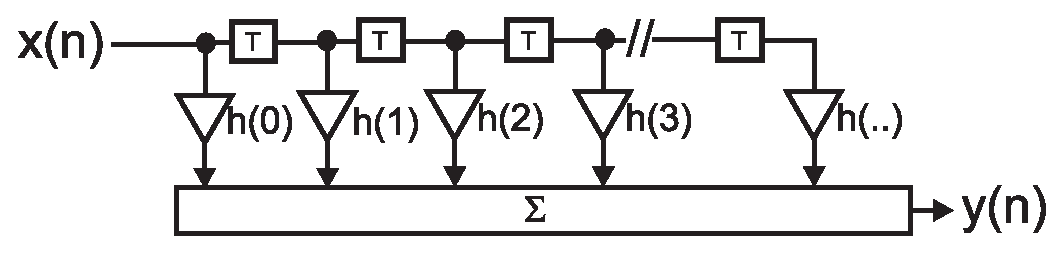
\includegraphics[width=\linewidth]{fir_digital}}
\caption{Digital FIR filter with normalised frequency \label{fir_digital}}
\end{center}
\end{figure}

This is the formula of an Finite Impulse Response filter where we have
sampled an analogue impulse response $h(t)$ at time intervals of $T$.
However, usually the impulse response of the filter is directly derived
in the digital domain where the argument $n$ of $h(n)$ represents just the sample
index $n$ and the sampling interval is implicitly the inverse of the sampling
rate. For that reason one needs to distinguish between:

\begin{eqnarray}
H(z)X(z) & = & \sum_{m=0}^M h_\textrm{\footnotesize{analogue}}(mT) z^{-n} \, X(z) \label{FIRa} \\
H(z)X(z) & = & \sum_{m=0}^M h_\textrm{\footnotesize{digital}}(m) z^{-n} \, X(z) \label{FIRd} \\
         & = & \sum_{m=0}^M h_(m) z^{-m} \, X(z) \label{FIRdefault}
\end{eqnarray}

Eq~\ref{FIRa} is the filter where the impulse response is based on an analogue
filter and Eq.~\ref{FIRd} is based on the impulse response originating from a digital filter
design (see section~\ref{freqsamp} and \ref{idealFilt}) where the frequencies
are normalised frequencies from $0$ to $0.5$. From now on we will
always refer to the ``digital'' one (Eq.~\ref{FIRd}) and the subscript will be
omitted (Eq.~\ref{FIRdefault} \& Fig.~\ref{fir_digital}).

In the time domain the FIR filter is then doing the following operation:
\begin{equation}
  y(n) = \sum_{m=0}^{M-1} h(m) x(n-m) \label{FIRtime}
\end{equation}

\subsubsection{Generally FIR filters do not perform a convolution operation}

Remember that we have derived the FIR filters from the analogue domain
by filtering a signal (Eq.\ref{notFIRyet}). The timedomain
representation of this is a discrete and causal convolution operation
(using the sampled Laplace transform). However, the problem is that
this runs to \textsl{infinite time} (see Eq~\ref{FIRtime}) and would
require an infinite number of delay steps and thus infinite time to
complete. So the FIR filter at best performs an approximation of the
convolution operation but there are serious problems with the finite
number of taps ($N$) which requires a technique called windowing which
moves it even further away from a convolution operation. On the other
hand if the impulse response is strictly limited in time one can use
this property for example for matched filters. However, the bottomline
is that sweeping statements such as that ``FIR filters perform a
convolution'' are \textsl{generally wrong} if nothing is known of the
impulse response.



\subsubsection{FIR filter implementations}
No matter the design process the implementation is always the same: we
need a delay line for the incoming signal and then weight the delayed
outputs by the different coefficients and for that reason are called
(water-) ``taps'' (see Eqs.~\ref{FIRa} \& \ref{FIRd}). We are now presenting
different implementations.

\begin{itemize}
\item C++:
This is a simple example of a filter which stores the values
in a simple linear buffer \texttt{bufferFIR} which stores the
delayed values. The coefficients are stored in \texttt{coeffFIR}.
\begin{verbatim}
  float filter(float value) {
    // shift
    for (int i=taps-1;i>0;i--)  {
      bufferFIR[i]=bufferFIR[i-l];
    }
    //store new value
    bufferFIR[0]=value;
    //calculate result
    for (int i=0;i<taps;i++)  {
      output +=bufferFIR[i]*coeffFIR[i];
    }
  return output;
  }
\end{verbatim}

\item Python: Here, the FIR filter is implemented as a
  class which receives the FIR filter coefficients
  in the constructor and then filters a signal sample
  by sample in the function filter:
  
\begin{verbatim}
class FIR_filter:
    def __init__(self,_coefficients):
        self.ntaps = len(_coefficients)
        self.coefficients = _coefficients
        self.buffer = np.zeros(self.ntaps)

    def filter(self,v):
        self.buffer = np.roll(self.buffer,1)
        self.buffer[0] = v
        return np.inner(self.buffer,self.coefficients)
\end{verbatim}
which again processes the signal sample by sample. It uses
the numpy ``roll'' command to shift the samples and then
the inner product to calculate the weighted sum between
the buffer and the coefficients.

If one wants
to filter a whole array one can use Python's lfilter command:
\begin{verbatim}
import scipy.signal as signal
y = signal.lfilter(h,1,x)
\end{verbatim}
This filters the signal \texttt{x} with the impulse response
\texttt{h}. Note that this operation is on an array and thus
a-causal.
\end{itemize}
More sophisticated code can be found in \citet{NumericalRec2007}.
This book is strongly recommended for any C programmer who
needs efficient solutions.


\subsubsection{Fixed point FIR filters}
\begin{figure}[!hbt]
\begin{center}
\mbox{\includegraphics[width=\linewidth]{fir_fixed}}
\caption{Fixed point FIR filter. The output signal is bit shifted to the
  right by $w$ bits while the coefficients are scaled up by $2^w$. \label{fir_fixed}}
\end{center}
\end{figure}
These filters receive integer numbers as input, perform integer multiplications/additions
and their outputs are integer as well. Thus, these filters do not require
a floating point unit on a processor.

Fig.~\ref{fir_fixed} shows a fixed point FIR filter. The input $x(n)$ is an integer
variable with I bit integers, the accumulator is an integer variable with A bits and
the output as well (usually the same as the input in terms of bit width).

In contrast to a floating point FIR filter we need to scale up the
coefficients so that they use full the integer range to avoid
quantisation errors. For example if the coefficients of $h(n)$ range
from $-0.75$ and $+0.75$ and we have signed 16 bit integers then the
scaling factor is $2^W, W=15$.

However, the accumulator A which collects the data needs to have more
bits because it receives scaled input values at I bits precision and
these multiplied by factor $2^W$. If we have $M$ taps then the additional
bits we need is $\log_2 M$. The total number of bits we need in the accumulator
in the worst case are:
\begin{equation}
  A = I + W + \log_2 M
\end{equation}
However, this is the worst case scenario because if the gain of the
FIR filter is below one then the summations by the $M$ taps will only
create \textsl{temporary} overflows because integer numbers are
cyclic in their representation. In case the gain of the FIR filter
is below one this can be relaxed:
\begin{equation}
  A = I + W
\end{equation}
The actual bitwidth of the accumulator is usually the next integer size
available and also makes sure that in case the gain goes slightly over one
in an unexpected case that the filter still works. For example if I
has $16$~bits the accumulator has probably $32$~bits.


\subsubsection{Constant group delay or linear phase filter}
So far the FIR filter has
no constant group delay which is defined by:
\begin{equation}
\tau_\omega= - {d\phi(\omega)\over d\omega}
\label{grpdelay}
\end{equation}
This means that different frequencies arrive at the output of the
filter earlier or later. This is not desirable. The group delay
$\tau_\omega$ should be constant for all frequencies $\omega$ so that
all frequencies arrive at the same time at the output $y$ of the
filter.

A constant group delay can be achieved by restricting ourselves to
the transfer function:
\begin{equation}
H(e^{i\omega})=B(\omega)e^{-i\omega\tau+i\phi} \label{transmin}
\end{equation}
where $B(\omega)$ is real and the phase is only defined by the exponential.
The phase of this transfer function is then trivially $\omega\tau+\phi$. The
group delay is the derivative of this term which is constant.

Eq.~\ref{transmin} now imposes restrictions on the impulse response $h(t)$
of the filter. To show this we use the inverse Fourier transform of
Eq.~\ref{transmin} to get the impulse response:
\begin{equation}
h(n)=\frac{1}{2\pi}\int_{-\infty}^{+\infty} H(e^{i\omega})
e^{i\omega n}d \omega
\end{equation}
After some transformations we get:
\begin{equation}
h(n+\tau)=\frac{1}{2\pi}e^{i\phi}b(n) \label{imp1}
\end{equation}
where $b(n)$ represents the Fourier coefficients of $B(\omega)$. Since $B$ is
real the coefficients $b(n)$ have the property $b(n)=b^*(-n)$.
Thus we get a second impulse response:
\begin{equation}
h(n+\tau)=\frac{1}{2\pi}e^{i\phi}b^*(-n) \label{imp2}
\end{equation}
Now we can eliminate $b$ by equating Eq.~\ref{imp1} and Eq.~\ref{imp2} which
yields:
\begin{equation}
h(n+\tau)=e^{2i\phi} n^*(-n+\tau)
\end{equation}
With the shift $\tau$ we have the chance to make the filter ``more''
causal. We can shift the impulse response in positive time to get
$h(n)$ zero for $n<0$. In a practical application we shift the impulse
response by half the number of delays. If we have a filter with $M$
taps we have to delay by $\tau=M/2$.

The factor $e^{2i\phi}$ restricts the values of $\phi$ because the impulse
response must be real. This gives us the final FIR design rule:
\begin{equation}
h(n+M/2)=(-1)^k h(-n+M/2)
\end{equation}
where $k=0$ or $1$. This means that the filter is either symmetric or
antisymmetric and the impulse response has to be delayed by $\tau=M/2$.




\subsubsection{Window functions}
\begin{figure}[!hbt]
\begin{center}
\mbox{\includegraphics[width=\linewidth]{window_functions}}
\caption{Different window functions applied to a low pass filter 
(Eq.~\ref{idealLP}) 
with cutoff at $f=0.1$ and 100 taps. \label{window_functions}}
\end{center}
\end{figure}
So far we still have a infinite number of coefficients for 
for the FIR filter because there's no guarantee that the 
impulse response becomes zero
after $M/2$ delays. Thus, we have to find a way to truncate the
response without distorting the filter response.

The standard technique is to multiply the coefficients with a window
function which becomes and stays zero at a certain coefficient
$n>N$ so that Eq.~\ref{FIRfromAnalogue} need not to run to infinity:
\begin{equation}
\label{FIRzlimit}
H(z)X(z)=\sum_{n=0}^N \underbrace{h(nT) w(nT)} z^{-n} X(z)
\end{equation}

\begin{enumerate}
\item Rectangular window: truncating the impulse response.
Problem: we get ripples in the frequency-response.
The stop-band damping is poor

\item Triangular or Bartlett window: greatly improved stop-band attenuation.
\item Hanning and Hamming window: standard windows in many applications.
\begin{equation}
w(n) = \alpha - (1-\alpha) \cos\left(\frac{2\pi n}{M}\right)
\end{equation}
\begin{itemize}
\item Hamming: $\alpha = 0.54$
\item Hanning: $\alpha = 0.5$
\end{itemize}

\item Blackman window:
\begin{equation}
w(n) = 0.42 + 0.5 \cos \left(\frac{2 \pi n}{M}\right) + 
0.08 \cos \left( \frac{4 \pi n}{M} \right) 
\end{equation}
\item Kaiser window: control over stop- and passband. No closed form
equation available.
\end{enumerate}
To illustrate how window functions influence the frequency response
we have taken an impulse response of a lowpass filter ($f_c=0.1$)
and applied different window functions to it (Fig.~\ref{window_functions}).

Note that the higher the damping the wider the transition from pass-
to stopband. This can be seen when comparing the Blackman window with
the Hamming window (Fig.~\ref{window_functions}). For the lowpass
filter this seems to be quite similar. However, for a bandstop filter
the wider transition width might lead actually to very poor stopband
damping. In such a case a Hamming window might be a better choice.


\subsubsection{Python code: 
impulse response from the inverse DFT - The frequency sampling
method\label{freqsamp}} Imagine that we want to remove $50Hz$ from a
signal with sampling rate of $1kHz$. We define an FIR filter with 100
taps. The midpoint $N/2=50$ corresponds to $500Hz$. The $50Hz$
correspond to index $5$.
\begin{verbatim}
f_resp=np.ones(100)
# note we need to add "+1" to the end because the end of
# the range is not included.
f_resp[4:6+1]=0
f_resp[94:96+1]=0
hc=np.fft.ifft(f_resp)
h=np.real(hc)
# this is from index 0 to index 49 on the left
# and on the right hand side from index 50 to index 99
h_shift[0:50]=h[50:100]
h_shift[50:100]=h[0:50]
h_wind=h_shift*hamming(100)
\end{verbatim}
To get a nice symmetric impulse response we need to shift the
inverse around $50$ samples.


\subsubsection{FIR filter design from ideal frequency response --
The analytical way
\label{idealFilt}}
For many cases the impulse response can be calculated analytically.
The idea is always the same: define a function with the ideal frequency
response
\begin{equation}
|H(e^{j\omega})| = \underbrace{B(e^{j\omega})}_{\mbox{real}}
\end{equation}
and perform an inverse Fourier transform to get the impulse response
$h(n)$.

We demonstrate this with a lowpass filter:
\begin{equation}
|H(e^{j\omega})| =
\left\{
\begin{array}{ll}
1 & \mbox{for } |\omega| \leq \omega_{c} \\
0 & \mbox{for } \omega_c < |\omega| \leq \pi
\end{array}
\right.
\end{equation}

Use the inverse Fourier transform to get the impulse response:
\begin{eqnarray}
h(n) & = & \frac{1}{2 \pi} \int_{-\pi}^{\pi} H(e^{j \omega}) e^{j \omega n} d\omega \\
     & = & \frac{1}{2 \pi} \int_{- \omega_{c}}^{+ \omega_{c}} e^{j \omega n} d\omega \\
     & = & \frac{1}{2 \pi} \left[\frac{1}{jn} e^{j \omega n} \right]_{- \omega_{c}}^{+ \omega_{c}} \\
     & = & \frac{1}{2 \pi jn} \left( e^{j \omega_{c} n} - e^{-j \omega_{c}n} \right)
\end{eqnarray}
With these handy equations:
\begin{eqnarray}
\sin z & = & \frac{1}{2j} (e^{zj} - e^{-zj})\\
\cos z & = & \frac{1}{2} (e^{zj} + e^{-zj})
\end{eqnarray}
we get for the filter:
\begin{equation}
h(n) = 
\left\{
\begin{array}{cc}
\frac{1}{\pi n} \sin \omega_{c}n & \mbox{for } n \neq 0 \\
\frac{\omega_{c}}{\pi} & \mbox{for }n = 0
\end{array}
\right.
\end{equation}
This response is a-causal! However we know that we can shift the response 
by any number of samples to make it causal! And we have to window the
response to get rid of any remaining negative contribution and to
improve the frequency response.

Highpass, bandstop and bandpass can be calculated in exactly the same
way and lead to the following ideal filter characteristics:
\begin{itemize}
\item \textbf{Lowpass} with cutoff frequency $\omega_c=2\pi f_c$:
\begin{equation}
h(n) = 
\left\{
\begin{array}{ll}
\frac{\omega_c}{\pi} & \mbox{for $n=0$} \\
\frac{1}{\pi n} \sin(\omega_c n) & \mbox{for $n\neq 0$}
\end{array}
\right.
\label{idealLP}
\end{equation}

\item \textbf{Highpass} with the cutoff frequency $\omega_c=2\pi f_c$:
\begin{equation}
h(n)=
\left\{ 
\begin{array}{ll}
1-\frac{\omega_c}{\pi} & \mbox{for $n=0$} \\
-\frac{1}{\pi n} \sin(\omega_c n) & \mbox{for $n\neq 0$}
\end{array}
\right.
\end{equation}

\item \textbf{Bandpass} with the passband frequencies $\omega_{1,2}=2\pi f_{1,2}$:
\begin{equation}
h(n)=
\left\{ 
\begin{array}{ll}
\frac{\omega_2-\omega_1}{\pi} & \mbox{for $n=0$} \\
\frac{1}{\pi n}(\sin(\omega_2 n)-\sin(\omega_1 n)) & \mbox{for $n\neq 0$}
\end{array}
\right.
\end{equation}

\item \textbf{Bandstop} with the notch frequencies $\omega_{1,2}=2\pi f_{1,2}$:
\begin{equation}
h(n)=
\left\{ 
\begin{array}{ll}
1-\frac{\omega_2-\omega_1}{\pi} & \mbox{for $n=0$} \\
\frac{1}{\pi n}(\sin(\omega_1 n)-\sin(\omega_2 n)) & \mbox{for $n\neq 0$}
\end{array}
\right.
\end{equation}
\end{itemize}
See \citet[p.195]{Diniz2002} for more impulse responses.

Here is an example code for a bandstop filter which fills the array
\texttt{h} with the analytically calculated impulse response:
\begin{verbatim}
f1 = 45.0/fs
f2 = 55.0/fs
n = np.arange(-200,200)
h = (1/(n*np.pi))*(np.sin(f1*2*np.pi*n)-np.sin(f2*2*np.pi*n))
h[200] = 1-(f2*2*np.pi-f1*2*np.pi)/np.pi;
h = h * np.hamming(400)
\end{verbatim}
After the function has been calculated it is windowed so that the
cut off is smooth. It's not very elegant as it's causes a division by zero first and
then the coeffecient at 200 is fixed. Do it better!


\subsubsection{Design steps for FIR filters}
Here are the design steps for an $M$ tap FIR filter.
\begin{enumerate}
\item Get yourself an impulse response for your filter:
\begin{enumerate}
\item Create a frequency response ``by hand'' just by filling an array
with the desired frequency response. Then, perform an inverse Fourier transform
(see section~\ref{freqsamp}).
\item Define a frequency response analytically. Do an inverse Fourier
transform (see section~\ref{idealFilt}).
\item Use an analogue circuit, get its impulse response and use
these as filter coefficients.
\item Dream up directly an impulse response (for example, averagers,
differentiators, etc)
\end{enumerate}

\item Mirror the impulse response (if not already symmetrical)
\item Window the impulse response from an infinite number of samples
to $M$ samples.
\item Move the impulse response to positive time so that it becomes causal
(move it $M/2$ steps to the right).
\end{enumerate}



\subsubsection{FIR filter design with Python's high level functions}
The ``firwin'' command generates the impulse response of
a filter with m taps and also applies a default window function. For example:
\begin{verbatim}
from scipy.signal import firwin
h = firwin(m,2*f)
\end{verbatim}
generates a lowpass FIR filter with the normalised frequency f. Note the
factor two because in scipy the normalisation is \textsl{not} the sampling rate
but the \textsl{nyquist frequency}. To be compatible with the math here the
easiest approach is to multiply the frequency by 2. With this command
one can also design high pass, bandstop and bandpass filters. Type \texttt{help(firwin)}
which provides examples for all filter types and which parameters need
to be set.



\subsubsection{Signal Detection: Matched filter}
How can I detect a certain event in a signal? With a correlator.
Definition of a correlator?
\begin{equation}
e(t) = \int_{0}^{t} \underbrace{s(\tau)}_{\mbox{signal}} \underbrace{r(\tau)}_{\mbox{template}} d(\tau)
\end{equation}

How to build a correlator with a filter? Definition of filtering?

\begin{equation}
e(t) = \int_{0}^{\infty} s(\tau) h(t - \tau) d\tau 
\end{equation}
NB. h - integration runs backwards.  However we used an int forward!
$h(t) : = r(T - \tau)$, only valid for $0\ldots T$.

\begin{eqnarray} 
e(t) & = & \int_{0}^{T} s(\tau) r \left(T - (t - \tau)\right) d\tau \\
     & = & \int_{0}^{T} s(\tau) r(T - t + \tau) d\tau 
\end{eqnarray}
for $t: = T$ we get:
\begin{equation}
e(T) = \int_{0}^{\infty} s(\tau) r (\tau) d\tau
\end{equation}
\begin{equation}
\underbrace{h(t) : = r(T - t)}_{ matched \quad  filter!} 
\end{equation}
In order to design a detector we just create an impulse
response $h$ by reversing the template $r$ in time and
constructing an FIR filter with it.

How to improve the matching process? Square the output of the filter!

\subsubsection{Adaptive FIR Least Mean Squares (LMS) filters}
\begin{figure}[!hbt]
\begin{center}
\mbox{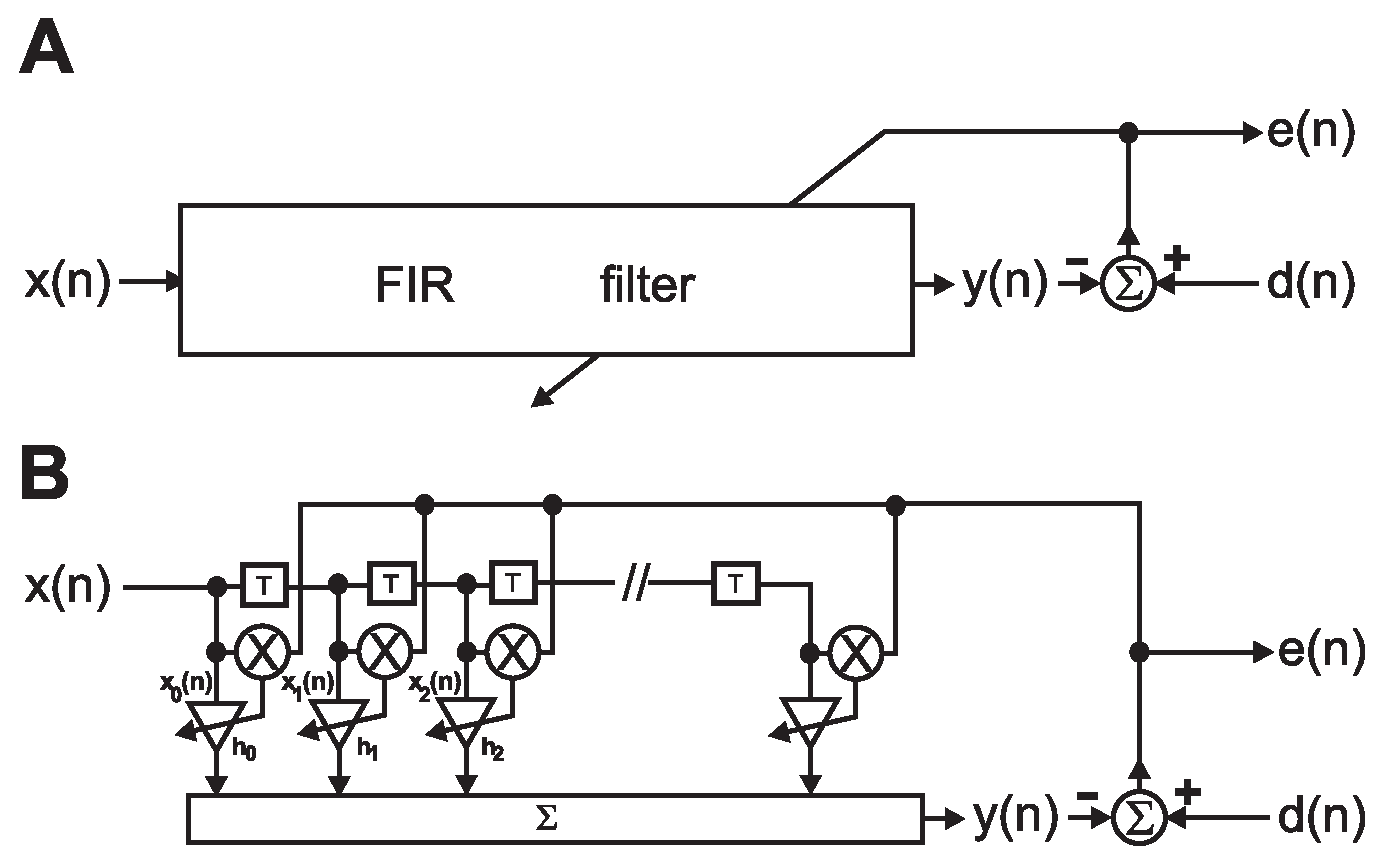
\includegraphics[width=\linewidth]{fir_lms}}
\caption{Adaptive FIR filter \label{fir_lms}: A) Negative feedback
  loop where a desired signal $d(n)$ is compared with the output
  of the FIR filter $y(n)$ and creates the error signal $e(n)$ which
  then tunes the FIR filter. B) Internal workings of the adaptive FIR
  filter where the error signal $e(n)$ is multiplied with the delayed input signal
  $x(n-m)$ and then changes the FIR filter coefficients $h_m$.}
\end{center}
\end{figure}
So far the coefficients of the FIR filter have been constant but now
we are going to allow them to change \textsl{while} the FIR filter is
operating so that it can learn its own coefficients. The
idea is to use an error signal $e(n)$ to tune the coefficients $h(n)$
of the FIR filter (see Fig.~\ref{fir_lms}A) by comparing its output
$y(n)$ with a desired output $d(n)$:
\begin{equation}
  e(n) = d(n) - y(n) \label{lmserror}
\end{equation}
and tuning the FIR filter in a negative feedback loop till the
average of $e(n)$ is zero.

We need to derive how the error $e(n)$ can change the FIR filter
coefficients so that the error is actually minimised. This can be
expressed as a so called ``gradient descent'' which minimises the squared
error $\frac{1}{2} e(n)^2$ because both a positive and a negative
error are equally bad:
\begin{equation}
  \Delta h_m = - \mu \frac{\partial\left( \frac{1}{2}e(n)^2 \right)}{\partial h_m} \label{graddes}
\end{equation}
where $\Delta h_m(n)$ is the change of the coefficient $h_m(n)$ at
every time step: $h_m(n+1) = h_m(n) + \Delta h_m(n)$.  $\mu \ll 1$
defines how quickly the coefficients $h_m$ change at every time step
and is called the ``learning rate''. Note here the change in notation
of the FIR filter coefficients $h_m$ which are changing much
\textsl{slower} than the sampled signals $e(n), d(n)$ and $y(n)$ and
can still be seen as constant for the realtime filtering
operation. Thus, we have $n$ for the sample by sample processing as
before and the index $m$ of $h_m$ for the very slowly changing FIR
filter coefficients. To gain some intuition why
Eq.~\ref{graddes} mimimises the error $e(n)$ we look at what happens if we
increase the FIR coefficient $h_m$ a little bit, for example, by the
small amount of $|\epsilon| \ll 1$: $h_m := h_m + \epsilon$. Then we can
observe two cases:
\begin{enumerate}
\item The squared error $e(n)^2$ increases so we need to decrease $h_m$ as it makes it worse.
\item The squared error $e(n)^2$ decreases so we need to increase $h_m$ as it makes it better.
\end{enumerate}
This also works in the same way if we decrease $h_m$ by a small amount. Thus from
both directions this always minimises the error. This is basically a carrot \& stick
approach where the coefficients $h_m$ are being ``rewarded'' if they minimise the error and
``punished'' if they make the error larger. This approach is called ``Least Mean Squares'' (LMS)
as it minimises the squared error on average. It's also known from neural networks where
the $h_m$ are called the ``weights'' of a neuron (see delta rule).

Eq~\ref{graddes} now needs to be turned into a form which can directly run in software by
solving its partial derivative by inserting Eqs.~\ref{lmserror} and \ref{FIRtime}.
\begin{eqnarray}
  \Delta h_m & = & - \mu \frac{1}{2}\frac{\partial \left(d(n)-y(n)\right)^2}{\partial h_m} \\
                & = & - \mu \frac{1}{2}\frac{\partial \left(d(n)-\sum_{m=0}^{M-1} h_m \cdot x(n-m)\right)^2}{\partial h_m} \\
                & = & \mu \left(d(n)-y(n)\right) \cdot x(n-m) \\
                & = & \mu \cdot e(n) \cdot x(n-m) \label{lmsLearn}
\end{eqnarray}
Note that $x(n-m)$ emerges because
of the chain rule when partially differentiating the output
$y(n)$ which depends on the sum of the delay lines of the FIR
filter (see Eq~\ref{FIRtime}). Eq.~\ref{lmsLearn} is now our ``learning''
rule which can simply be applied to the FIR filter as showm in Fig~\ref{fir_lms}B.

Now we have the recipe of an adaptive filter where the FIR filter minimises its
own error $e(n)$ in a negative feedback loop and generating an output
$y(n)$ which is as closely as possible to the desired signal $d(n)$. The signal
$y(n)$ is often called ``the remover'' as it cancels out the signal $d(n)$.
However, not everything in $d(n)$ is cancelled out but \textsl{only} what
is correlated with the input $x(n)$. This means that the error signal
$e(n)$ will not be zero but will contain any signal components which are
\textsl{not} correlated with $x(n)$. This means that the error signal actually
is also the cleaned up output signal of the adaptive filter.

Imagine you want to remove $50$~Hz mains from a signal
\begin{equation}
d(n) = \mathrm{signal}(n) + \mathrm{50Hz~noise}(n)
\end{equation}
then one would provide $50$~Hz mains
via
\begin{equation}
  x(n) = \mathrm{50Hz~noise}(n)
\end{equation}  
so that then the filter learns to remove the powerline
interference. One might think that the filter will remove everything from
$d(n)$ because it will try to minimise the error $e(n)$ but only the
50~Hz in the contaminated signal will be removed because only signal components
which are correlated between $x(n)$ and $d(n)$ will be removed.
The cleaned up signal will be identical to the error
signal:
\begin{equation}
  e(n) = \mathrm{signal}(n)
\end{equation}


\clearpage
\subsection{IIR Filter}
IIR filter stands for Infinite Impulse Response. Such filters have
feedback so that signals are processed in a recursive way. We will see
that impulse responses from exponentials can easily be implemented as
a recursive filter.

\subsubsection{Introduction}
As an instructional example we take a very simple analogue filter and
sample it. This can then be generalised to more complex
situations.

We define a first order filter which can be implemented, for example, as
a simple RC network:
\begin{equation}
h(t)=e^{-bt}
\label{ExpoFunktion}
\end{equation}
where its Laplace transform is a simple fraction:
\begin{equation}
H(s)=\frac{1}{s+b}
\end{equation}
Now we sample Eq.~\ref{ExpoFunktion}:
\begin{equation}
h(t)=\sum_{n=0}^\infty e^{-bnT} \cdot \delta(t-nT)
\end{equation}
and perform a Laplace transform on it:
\begin{equation}
H(s) = \sum_{n=0}^\infty e^{-bnT} \underbrace{e^{-nsT}}_{{z^{-1}}^n}
\end{equation}
which turns into a z-transform:
\begin{eqnarray}
H(z)&=&\sum_{n=0}^\infty e^{-bnT} z^{-n} \\
    &=&\sum_{n=0}^\infty {\left(e^{-bT} z^{-1}\right)}^n \\
    &=&{1\over 1-e^{-bT} z^{-1}}  \label{IIReq}
\end{eqnarray}
Consequently the analogue transfer function $H(s)$
transfers into $H(z)$ with the following recipe:
\begin{equation}
H(s)=\frac{1}{s+b} \qquad\Leftrightarrow\qquad
H(z)=\frac{1}{1-e^{-bT} z^{-1}} \label{impInv}
\end{equation}
Thus, if you have the poles of an analogue system and you want
to have the poles in the z-plane you can transfer them with:
\begin{equation}
z_\infty=e^{s_\infty T}
\label{translpoles}
\end{equation}
This also gives us a stability criterion. In the Laplace domain
the poles have to be in the left half plane (real value negative).
This means that in the sampled domain the poles have to lie within
the unit circle.

The same rule can be applied to zeros
\begin{equation}
z_0=e^{s_0 T} \label{transzeros}
\end{equation}
together with Eq.~\ref{translpoles} this is called ``The matched
z-transform method''. For example $H(s)=s$ turns into
$H(z)=1-z^{-1}e^{0T}=1-z^{-1}$ which is basically a DC filter.


\subsubsection{Determining the data-flow diagram of an IIR filter}
\begin{figure}[!hbt]
\begin{center}
\mbox{\includegraphics[width=0.75\linewidth]{iir}}
\caption{IIR filter \label{IIRfilter}}
\end{center}
\end{figure}
To get a practical implementation of Eq.~\ref{IIReq} we have
to see it with its input- and output-signals:
\begin{eqnarray}
Y(z)&=&X(z)H(z)\\
    &=&X(z) {1\over 1-e^{-bT} z^{-1}} \\
    &=&Y(z)z^{-1}e^{-bT}+X(z)
\label{Verg}
\end{eqnarray}
We have to recall that $z^{-1}$ is the delay by $T$. With that
information we directly have a difference equation in the
temporal domain:
\begin{equation}
y(nT)=y([n-1]T) e^{-bT} + x(nT)
\label{IIRtime}
\end{equation}
This means that the output signal $y(nT)$ is calculated by
adding the weighted and delayed output signal $y([n-1]T)$ 
to the input signal $x(nT)$.
How this actually works is shown in Fig.~\ref{IIRfilter}.
The attention is drawn to the \textsl{sign inversion} of the weighting
factor $e^{-bT}$ in contrast to the transfer function 
Eq.~\ref{impInv} where it is $-e^{-bT}$. In general the recursive
coefficients change sign when they are taken from the transfer
function.



\subsubsection{General form of IIR filters}
A filter with forward and feedback components can be represented as:
\begin{equation} 
H(z) = \frac{\sum_{k = 0}^{r} B_{k} z^{-k}}{1 + \sum_{l = 1}^{m} A_{i} z^{-l}} \end{equation}
where $B_k$ are the FIR coefficients and $A_l$ the recursive coefficients.
Note the signs of the recursive coefficients are \textsl{inverted} in the
actual implementation of the filter. This can be seen when the
function $H(z)$ is actually multiplied with an input signal to
obtain the output signal (see Eq.~\ref{IIRtime} and Fig.~\ref{IIRfilter}).
The ``1'' in the denominator represents actually the output of
the filter. If this factor is not one then the output will be scaled
by that factor. However, usually this is kept one.

In Python filtering is performed with the command:
\begin{verbatim}
import scipy.signal as signal
Y = signal.lfilter(B,A,X)
\end{verbatim}
where B are the FIR coefficients, A the IIR coefficients and X is the input.
For a pure FIR filter we just have:
\begin{verbatim}
Y = signal.lfilter(B,1,X)
\end{verbatim}
The ``1'' represents the output.


\subsubsection{IIR filter topologies}
\begin{figure}[!hbt]
\begin{center}
\mbox{\includegraphics[width=\textwidth]{iir_types}}
\end{center}
\caption{A) Direct Form I filter which one accumulator and
  B) Direct Form II filter with two accumlators.
\label{iir_types}}
\end{figure}
In real applications one would create a \textsl{chain of 2nd order
IIR filters}. This has numerous advantages:
\begin{enumerate}
\item The optimisation can be done within these simple structures,
  for example omitting array operations completely and coding
  the 2nd order filters in assembly while keeping the higher
  level operations in C or C++.
\item Control of stability issues: high order recursive
  systems might become unstable and it is very hard to predict
  when this might happen. On the other hand a chain of 2nd order
  filters can be made stable with ease. One can focus on
  stability in 2nd order systems which is well understood and
  manageable.
\item Complex conjugate pole pairs are generated naturally
  in analogue filter design and directly translate to 2nd
  order IIR structures. Analogue design is usually described
  as 2nd order structures (=LCR) so that any transform from analogue
  to digital just needs to be of 2nd order!
\end{enumerate}

Fig.~\ref{iir_types} shows the most popular filter topologies:
Direct Form I and II. Because of the linear operation of the filter
one is allowed to do the FIR and IIR operations in different orders.
In Direct From I we have one accumulator and two delay lines whereas
in the Direct Form II we have two accumulators and one delay line.
Only the Direct Form I is suitable for integer operations.

A Python class of a direct form II filter can be implemented
with a few lines:
\begin{verbatim}
class IIR_filter:
    def __init__(self,_num,_den):
        self.numerator = _num
        self.denominator = _den
        self.buffer1 = 0
        self.buffer2 = 0

    def filter(self,v):
        input=0.0
        output=0.0
        input=v
        output=(self.numerator[1]*self.buffer1)
        input=input-(self.denominator[1]*self.buffer1)
        output=output+(self.numerator[2]*self.buffer2)
        input=input-(self.denominator[2]*self.buffer2)
        output=output+input*self.numerator[0]
        self.buffer2=self.buffer1
        self.buffer1=input
        return output
\end{verbatim}
Here, the two delay steps are represented by two variables
\texttt{buffer1} and \texttt{buffer2}.

In order to achive higher order filters one can then just
chain these 2nd order filters. In Python this can be achieved
by storing these in an array of instances of this class.

\subsubsection{Fixed point IIR filters}
\begin{figure}[!hbt]
\begin{center}
\mbox{\includegraphics[width=0.5\textwidth]{iir_fixed}}
\end{center}
\caption{Direct Form I filter with fixed point arithmetic.
\label{iir_fixed}}
\end{figure}
Fig.~\ref{iir_fixed} shows the implementation of a fixed point IIR
filter. It's a Direct Form I filter with one accumulator so that
temporary overflows can be compensated. The original floating point
IIR coefficients are scaled up by factor $2^w$ so that they max out
the range of the integer coefficients. After the addition operation
they are shifted back by $w$~bits to their original values.

For example if the largest IIR coefficient is 1.9 and we use 16 bit
signed numbers (max number is 32767) then one could multiply all
coefficients with $2^{14}$.

Then one needs to assess the maximum value in the accumulator which
is much more difficult than for FIR filters. For example,
resonators can generate high output values with even small input values
so that it's advisable to have a large overhead in the accumulator.
For example if the input signal is $16$~bit and the scaling factor is
$14$~bits then the signal will certainly occupy $16+14=30$~bits. With
an accumulator of 32 bits that gives only a headroom of 2~bits so the
output can only be 4 times larger than the input. A 64 bit accumulator
is a safe bet.

\subsubsection{Filter design based on analogue filters}
\begin{figure}[!hbt]
\begin{center}
\mbox{\includegraphics[width=0.5\textwidth]{butterworth_poles}}
\end{center}
\caption{Pole placements of the Butterworth filter. Its analogue
  cutoff frequency is $\Omega = 2\pi F$ where $F$ is the
  analogue cutoff frequency in Hertz. This filter can be implemented
  as a chain of 2nd order IIR filters (biquads) by using the
  complex conjugate pairs for the different 2nd order IIR filters.
\label{butterworth_poles}}
\end{figure}
Most IIR filters are designed from analogue filters by transforming
from the continuous domain ($h(t),H(s)$) to the sampled domain
($h(n),H(z)$).

\paragraph{A list of popular analogue transfer functions being
used for IIR filter design:}

\begin{itemize}
\item {\bf Butterworth:} All poles lie on the left half plane
  equally distributed on a half circle with radius $\Omega = 2\pi F$ which
  is shown in Fig.~\ref{butterworth_poles}. The Butterworth filter
  is by far the most popular filter. Here are its properties:
\begin{itemize} 
\item monotonic frequency response
\item only poles, no zeros
\item the Poles have analytical solution and very easy to calculate
\item no constant group delay but usually acceptable deviation from
  a strict constant group delay for many applications.
\end{itemize}

\item {\bf Chebyshev Filters:}
\begin{equation} 
|H(\Omega)|^{2} = \frac{1}{1 - \varepsilon^{2} T_{N} (\Omega/\Omega_{p})}
\end{equation}
where T = Chebyslev polynomials. These filters have either ripples
in the stop or passband depending on the choice of polynomials.
As with Butterworth the polynomials have analytical solutions for
the poles and zeros of the filter so that their design again is
straightforward.

\item {\bf Bessel Filter: }
\begin{itemize} 
\item Constant Group Delay
\item Shallow transition from stop- to passband
\item No analytical solution for the poles/zeros.
\end{itemize}
\end{itemize}

\paragraph{How to transform the analogue lowpass filters into
  highpass, bandstop or bandpass filters?}
All the analogue transfer functions above are lowpass
filters. However this is not a limitation because there are handy transforms
which take an analogue lowpass transfer function or poles/zeros
and then transforms them into highpass, bandpass and stopband
filters. These rules can be found in any good analogue filter
design book and industry handouts, for example from Analog Devices.

\paragraph{Bilinear Transform: transforming the analoge transfer function into a digital one:}
As a next step these analogue transfer functions $H(s)$ need to be
transformed to digital transfer functions $H(z)$. This could be done
by the matched z-transform. However, the problem with these methods is that
they map frequencies 1:1 between the digital and analogue
domain. Remember: in the sampled domain there is no infinite frequency
but $F_s/2$ which is the Nyquist frequency.  This means that we never
get more damping than at Nyquist $F_s/2$.  This is especially a
problem for lowpass filters where damping increases the higher the
frequency.

The solution is to map {\bf all} analogue frequencies from $0 \ldots \infty$
to the sampled frequencies $0\ldots 0.5$ in a non-linear way:
\begin{equation} 
- \infty < \Omega < \infty \Rightarrow -\pi \leq \omega \leq \pi 
\end{equation}
This is called \textsl{Bilinear Transformation}:
\begin{equation} 
s = \frac{2}{T} \quad \frac{z - 1}{z + 1}
\end{equation}
This rule replaces all $s$ with $z$ in our analogue transfer
function so that it's now digital. However, the cutoff frequency $\Omega_c$
is still an analogue one but if we want to design a digital filter
we want to specify a digital cutoff frequency. Plus remember that
the frequency mapping is non-linear so that there is non-linear
mapping also of the cutoff. 

In the analogue domain the
frequency is given as $s = j\Omega$ and in the sampled domain as
$z = e^{j \omega}$. With the definition of the bilinear transform
we can establish how to map from our desired digital cutoff to
the analogue one:
\begin{equation} 
j \Omega = \frac{2}{T} \left[\frac{e^{j \omega} - 1}{e^{j \omega} +1}\right] = \frac{2}{T} j \tan \frac{\omega}{2}
\end{equation}
This derivation is useful for two purposes. It shows the non-linear
mapping between the digital and analogue world and it provides
a recipe how to calculate our analogue cutoff frequency.

That the bilinear transform is a 
{\bf non}linear mapping between the analogue world and the digital
world can be directly seen by just omitting the $j$:
\begin{equation}
\Omega = \frac{2}{T} tan \frac{\omega}{2}
\end{equation}

This also means that the cut-off frequency of our analogue filter is changed
by the bilinear transformation. Consequently, we need to apply the same
transformation to the cutoff frequency itself:
\begin{equation}
\Omega_{c} = \frac{2}{T} tan \frac {\omega_{c}}{2}
\label{prewarp}
\end{equation}
where $T$ is the sampling interval. This is often called ``pre-warp''
but is simply the application of the same rule to the cut-off
frequency as what the bilinear transform does to the transfer function
$H(s)$. It has also another important result: we can now finally
specify our cut-off in the sampled domain in normalised frequencies
$\omega_{c} = 2\pi f_{c}$ by using Eq.~\ref{prewarp}. After all we
just use the analogue filter as a vehicle to design a digital filter.

We can now list our design steps.

\paragraph{IIR filter design steps:}
\begin{enumerate}
\item Choose the cut-off frequency of your digital filter $\omega_{c}$.
\item Calculate the analogue cutoff frequency $\omega_{c} \rightarrow
  \Omega_{c}$ with Eq.~\ref{prewarp}
\item Choose your favourite analogue lowpass filter $H(s)$,
for example Butterworth.
\item Replace all $s$ in the analogue transfer function
$H(s)$ by $s = \frac{2}{T} \frac{z - 1}{z + 1}$ 
to obtain the digital filter $H(z)$
\item Change the transfer function $H(z)$ so that it only contains
negative powers of $z$ ($z^{-1}, z^{-2}, \ldots$) which can be
interpreted as delay lines.
\item Build your IIR filter!
\end{enumerate}

For filter-orders higher than two one needs to develop a different
strategy because the bilinear transform is a real \textsl{pain} to
calculate for anything above the order of two. Nobody wants to
transform high order analogue transfer functions $H(s)$ to the $H(z)$
domain. However, there is an important property of all analogue
transfer functions: they generate complex conjugate pole pairs (plus
one real pole if of of odd order) which suggest a chain of 2nd order IIR
filters straight away (see Fig.~\ref{butterworth_poles}). Remember
that a complex conjugate pole pair creates a 2nd order IIR filter with
with two delay steps. A real pole is a 1st order IIR filter with one
delay but is often also implemented as a 2nd order filter where the
coefficients of the 2nd delay are kept zero.

The design strategy is thus to split up the analogue transfer function
$H(s)$ in a chain of 2nd order filters $H(s) = H_1(s) H_2(s) H_3(s)
\ldots$ and then to apply the bilinear transform on every 2nd order
term separately. Using this strategy you only need to calculate the bilinear
transform once for a 2nd order system (or if the order is odd then
also for a 1st order one) but then there is no need to do any more
painful bilinear transforms. This is standard practise in IIR filter
design.

\paragraph{Time or frequency domain?}
The transforms from analogue to digital alter both the temporal
response and the frequency response. However the different transforms
have different impact. The bilinear transform guarantees that the
digital filter uses the whole frequency range of the analogue filter
from zero to infinity which is the best solution for frequency domain
problems. However, if one needs to reproduce the temporal response an
analogue filter as faithfully as possible then the matched z transform
is best because it's based (as the name suggests) on the impulse
invariance method which aims to preserve the temporal behaviour of the
filter (exact for pole-only transfer functions).

\begin{center}
\begin{tabular}{ll}
  Identical frequency response required: & Bilinear transform \\
  Identical temporal behaviour required: & Matched z-transform \\
\end{tabular}
\end{center}

Of course a 100\% match won't be achieved but in practise this
can be assumed. In most cases the bilinear transform is the
transform of choice. The matched z transform can be very useful,
for example in robotics where timing is important.



\subsubsection{Adaptive IIR filter: The Kalman filter}
Often signals are contaminated by high frequency noise where the
spectrum of the noise is changing or not known. The cutoff of a fixed low
pass filter is not known or might be changing so that we need to adapt the cut-off continuously.
One example is a Kalman filter which maximises the
\textsl{predictability} of the filtered signal. It's an adaptive lowpass filter
which increases the predictability of a signal because it smoothes it.
\begin{equation} 
H(z) = \frac{b}{1 - a z^{-1}}
\end{equation}
The parameter $a$ determines the cutoff frequency.
Frequency Response :
\begin{equation} 
|H(e^{j \omega}) | = |\frac{b}{1 - a e^{-j \omega}}| 
\end{equation}
Let's re-interpret our low-pass filter in the time domain:
\begin{equation} 
\underbrace{y(n)}_{\mbox {\footnotesize actual estimate}} = a(n) \underbrace{y(n - 1)}_{\mbox{\footnotesize previous estimate}} + b(n)\underbrace{x(n)}_{\mbox{\footnotesize current data sample}} 
\end{equation}
We would like to have the best estimate for $y(n)$
\begin{equation} 
p(n) = E[ \left( y (k) - y_{real} (k)\right)^{2}] 
\end{equation}
We need to minimise $p$ which gives us equations for a and b which
implements a Kalman filter.




\subsubsection{The role of poles and zeros}
Transfer functions contain poles and zeros. To gain a deeper
understanding of the transfer functions we need to understand
how poles and zeros shape the frequency response of $H(z)$.
The position of the poles also determines the stability of the filter
which is important for real world applications.

We are going to explore the roles of poles and zeros first with
an instructional example which leads to a 2nd order bandstop filter.

\paragraph{Zeros}
\begin{figure}[!hbt]
\begin{center}
\mbox{\includegraphics[width=0.75\textwidth]{fir_stop}}
\end{center}
\caption{A two tap FIR stopband filter for the frequency $\omega_0$.
\label{fir_stop}}
\end{figure}
Let's look at the transfer function:
\begin{eqnarray}
H(z) & = & (1 - e^{j\omega_0} z^{-1})(1 - e^{-j\omega_0} z^{-1}) \\
     & = & 1 - z^{-1} e^{j \omega-{0}} + z^{-2} \\
     & = & 1 - z^{-1} (e^{j \omega_{0}} + e^{-j \omega_{0}}) + z^{-2} \\
     & = & 1 - z^{-1} 2 \cos \omega_{0} + z^{-2}
\end{eqnarray}
which leads to the data flow diagram shown in Fig~\ref{fir_stop}.

\begin{equation}
H(e^{j\omega}) = \underbrace{(1 - e^{j\omega_0}e^{-j\omega})(1 - e^{-j\omega_0} e^{-j\omega})}_{\mbox{2 zeros}}
\end{equation}

The zeroes at 
$e^{j \omega_{0}}$ and $e^{-j \omega_0}$ 
eliminate the frequencies $\omega_{0}$ and $-\omega_{0}$. 

A special case is $\omega_{0} = 0$
which gives us:
\begin{eqnarray}
H(z) & = & (1 - e^{0} z^{-1})(1 - e^{0} z^{-1}) \\
     & = & 1 - 2 z^{-1} + z^{-2}
\end{eqnarray}
a DC filter.

In summary: zeros eliminate frequencies (and change phase).
That's the idea of an FIR filter where loads of zeros (or loads of taps)
knock out the frequencies in the stopband.


\paragraph{Poles}
\begin{figure}[!hbt]
\begin{center}
\mbox{\includegraphics[width=0.75\textwidth]{iir_stop}}
\end{center}
\caption{A two tap IIR resonator for the frequency $\omega_0$ and with
the amplification $r$.
\label{iir_stop}}
\end{figure}
While zeros knock out frequencies, poles amplify frequencies.
Let's investigate complex conjugate poles:
\begin{equation}
H(z) = \frac{1}{\underbrace{(1 - r e^{j \omega_{0}} z^{-1})(1 - r e^{-j \omega_{0}} z^{-1})}_{2 poles!}} 
\label{resonatorz}
\end{equation}
which are characterised by their resonance frequency $\omega_0$
and the amplification $0<r<1$.

In order to obtain a data flow diagram we need to get powers of $z^{-1}$
because they represent delays.
\begin{equation}
H(z) = \frac{1}{1 - 2 r \cos(\omega_{0}) z^{-1} + r^{2} z^{-2}} 
\end{equation}
which we multiply with the input signal $Y(z)$:
\begin{eqnarray} 
Y(z) & = & X(z) \frac{1}{1 - 2 r \cos (\omega) z^{-1} + r^{2} z^{-2}} \\
X(z) & = & Y(z) - Y(z) 2r \cos (\omega_{0}) z^{-1} + Y(z) r^{2} z^{-2} \\
Y(z) & = & X(z) + z^{-1} Y(z) 2r \cos (\omega_{0}) - z^{-2} Y(z) r^{2}
\end{eqnarray}
This gives us a second order recursive filter (IIR) which is
shown in Fig~\ref{iir_stop}. These complex
conjugate poles generate a resonance at $\pm\omega_0$ where the
amplitude is determined by $r$.

\paragraph{Stability}
A transfer function $H(z)$ is only stable if the poles lie inside the
unit circle. This is equivalent to the analog case where the poles of
$H(s)$ have to lie on the left hand side of the complex plane (see
Eq.~\ref{translpoles}). Looking at Eq.~\ref{resonatorz} it becomes
clear that $r$ determines the radius of the two complex conjugate poles. If
$r>1$ then the filter becomes unstable. The same applies to poles on
the real axis. Their the real values have to stay within the range $-1
\ldots +1$.

In summary: poles generate resonances and amplify frequencies. The
amplification is strongest the closer the poles move towards the unit
circle. The poles need to stay within the unit circle to guarantee
stability. 

Note that in real implementations the coefficients of the
filters are limited in precision. This means that a filter might
work perfectly in python but will fail on a DSP with its limited
precision. You can simlate this by forcing a certain datatype
in python or you write it properly in C.

\paragraph{Poles and zeroes combined: design of a pure digital IIR notch filter}
\begin{figure}[!hbt]
\begin{center}
\mbox{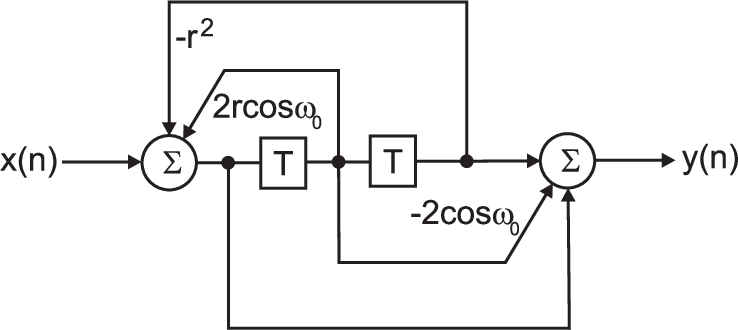
\includegraphics[width=0.75\textwidth]{iir_fir_stop}}
\end{center}
\caption{A two tap IIR bandstop filter with tuneable stopband width $r$
for the frequency $\omega_0$.
\label{iir_fir_stop}}
\end{figure}
Now we combine the filters from the last two sections:
\begin{equation} 
H(z) = \frac {1 - 2 \cos (\omega_{0}) z^{-1} + z^{-2}}{1 - 2r \cos (\omega_{0}) z^{-1} + r^{2} z^{-2}} 
\end{equation}
This gives us a notch filter where its width is tunable with the
help of $r<1$. The closer $r$ goes towards $1$ the more narrow
is the frequency response.
This filter has two poles and two zeros. The zeros sit on the unit
circle and eliminate the frequencies $\pm\omega_0$ while the
poles sit within the unit circle and generate a resonance around
$\pm\omega_0$. As long as $r<1$ this resonance will not go towards
infinity at $\pm\omega_0$ so that the zeros will always eliminate
the frequencies $\pm\omega_0$.

\paragraph{Identifying filters from their poles and zeroes}
\citet[pp.333]{Proakis1996} has an excellent section about this topic
and we refer the reader to have a look. As a rule of thumb a digital
lowpass filter has poles where their real parts are positive and a
highpass filter has poles with negative real part of the complex
poles. In both cases they reside within the unit circle to guarantee
stability.


\bibliographystyle{apalike}

\bibliography{laplace}

\end{document}
